
\chapter{Einleitung}\label{sec:Einleitung}

Das \emph{Semantic Web} erweitert das heutige Web um explizite Bedeutung: Inhalte werden so strukturiert, dass nicht nur Menschen, sondern auch Programme die Semantik verarbeiten und komplexe Aufgaben automatisiert unterstützen können \cite{bernersLee2001}. Dazu werden Informationen maschinenlesbar beschrieben (u.\,a.\ via URIs/IRIs und RDF-Tripeln), sodass Software-Agenten Datenquellen verbinden, Schlussfolgerungen ziehen und Dienste orchestrieren können—ohne zentrale Steuerung und im Sinne eines dezentralen, evolvierenden Webs \cite{bernersLee2001}.

Auf dieser Grundlage haben sich \emph{Wissensgraphen} als prägnante und flexible Datenabstraktion etabliert: Knoten repräsentieren Entitäten, Kanten ihre (auch komplexen) Relationen; Schemaentscheidungen können aufgeschoben, Datenquellen schrittweise integriert und Beziehungen über Pfade navigiert werden \cite{hogan2021}. Für RDF-basierte Wissensgraphen stellt \emph{SPARQL} die standardisierte Abfrage- und Änderungs\-sprache bereit. SPARQL operiert über Graphmuster (\emph{Basic Graph Patterns}) und unterstützt u.\,a.\ optionale/alternative Muster, Filter, Aggregation, Unterabfragen, Eigenschaftspfade sowie verschiedene Abfrageformen (SELECT, CONSTRUCT, ASK, DESCRIBE) \cite{w3cSparql11}. Trotz dieser Ausdrucksstärke bringt SPARQL inhärente Komplexität mit sich: Formal basiert es auf Graph-Matching; optionale Teile, UNION, FILTER, Projektion, DISTINCT/ORDER/LIMIT \emph{etc.} erhöhen die kognitive und algorithmische Schwierigkeit \cite{perezGutierrezSparql}. Für viele Endnutzer:innen bleibt die Syntax—und das Denken in Tripeln, Mustern und Bindungen—eine Hürde.

Parallel vergrößern \emph{Large Language Models (LLMs)} den Gestaltungsspielraum natürlicher Schnittstellen. GPT-4 zeigt, dass Modelle natürliche Sprache robust verarbeiten und in anspruchsvollen Benchmarks Leistungsniveaus nahe menschlicher Expert:innen erreichen können—bei bekannten Grenzen wie Halluzinationen und der Notwendigkeit geeigneter Sicherheitsmaßnahmen \cite{openaiGPT42023}. Dies legt nahe, natürliche Sprache als Interface zu RDF-Daten nutzbar zu machen: Benutzer:innen formulieren Aufgaben in Alltagssprache; ein LLM generiert daraus \emph{valide} SPARQL-Operationen.

Für reale, domänenspezifische Wissensgraphen (z.\,B.\ historische Personen, Orte, Organisationen) genügt es jedoch nicht, nur SELECT-Anfragen abzudecken. Gefordert ist die \emph{semantische Bearbeitung}—\textbf{INSERT}, \textbf{DELETE} und \textbf{UPDATE}—mit \emph{Nachvollziehbarkeit} und \emph{Sicherheit}. Dabei ist der \textbf{Datenschutz} zentral: Bei natürlicher Spracheingabe, Prompt-Kontext und beim Logging können personenbezogene Daten betroffen sein; die EU-DSGVO fordert u.\,a.\ Datenminimierung, Zweckbindung, Integrität/Vertraulichkeit und Rechenschaftspflicht \cite{euGDPR2016}. Privacy-by-Design ergibt sich hier u.\,a.\ durch die Beschränkung des Modellkontexts auf \emph{Ontologie statt Instanzdaten} sowie durch Pseudo\-nymisierung und strikte Aufbewahrungsregeln für Query-Logs.

\paragraph{Ziel der Arbeit.}
Diese Arbeit konzipiert, implementiert und evaluiert eine Schnittstelle, die \emph{natürliche Sprache} in \emph{valide SPARQL-Änderungsoperationen} überführt und Datenschutz sowie Nachvollziehbarkeit durchgängig verankert. Kernideen sind:
\begin{enumerate}
  \item LLM-gestützte Generierung mit \emph{Ontologie-Kontext} (Klassen/Properties) statt vollständiger Instanzdaten,
  \item \emph{Vorschau} und \emph{Erklärung} der betroffenen Tripel,
  \item \emph{schrittweise Bestätigung} und \emph{Undo},
  \item \emph{Protokollierung} mit Pseudonymisierung und klaren Lösch-/Aufbewahrungsregeln.
\end{enumerate}

\paragraph{Forschungsfragen.}
\begin{description}
  \item[RQ1:] Mit welcher Genauigkeit lassen sich natürliche \emph{Änderungsanweisungen} in \emph{syntaktisch valide} und \emph{semantisch korrekte} SPARQL-Operationen (INSERT/DELETE/UPDATE) überführen?
  \item[RQ2:] Wie wirken \emph{Privacy-by-Design}-Maßnahmen (Ontologie-Kontext, Pseudonymisierung von Logs) auf Datenschutz, Nachvollziehbarkeit und Nutzbarkeit?
  \item[RQ3:] Wie beurteilen Nutzer:innen die \emph{Benutzbarkeit} (Verständlichkeit von Vorschau/Erklärungen/Undo) im Vergleich zu handgeschriebenen Queries; welcher Overhead entsteht?
\end{description}

\paragraph{Beitrag und Aufbau.}
Die Arbeit liefert (i) eine \emph{Anforderungsanalyse} für NL{\textrightarrow}SPARQL-Änderungen unter DSGVO-Vorgaben, (ii) eine \emph{Architektur} mit Komponenten für Prompting/Parser, Generator, Validator, Executor, Logger und Visualizer, (iii) eine \emph{Referenzimplementierung} (Frontend/Backend, SPARQL-Endpoint) und (iv) eine \emph{Evaluation} auf einer domänennahen Wissensbasis. Kapitel~\ref{sec:theorie} fasst Grundlagen (RDF/OWL/SPARQL, LLMs, Datenschutz) zusammen; Kapitel~\ref{sec:related-work} diskutiert verwandte Arbeiten; Kapitel~\ref{sec:konzeption} beschreibt Anforderungsanalyse \& Konzeption; Kapitel~\ref{sec:implementierung} die Implementierung; Kapitel~\ref{sec:evaluation} die Evaluation; Kapitel~\ref{sec:fazit} schließt mit Fazit und Ausblick.





\chapter{Theoretischer Hintergrund}
\label{sec:theorie}

\section{Grundlagen des Semantic Web}
\label{sec:grundlagen-semantic-web}

\subsection{Motivation und Grundidee}

Das World Wide Web ist allgegenwärtig und wächst stetig; seine Stärken -- hohe Aktualität, globale Verfügbarkeit und niedrige Publikationsschwellen -- gehen zugleich mit Herausforderungen einher: heterogene Formate, fehlende Qualitätssicherung und vor allem eine \emph{mangelnde maschinelle Interpretierbarkeit} von Inhalten \cite{Hitzler}. Suchmaschinen mildern dies mit statistischen Verfahren, bleiben jedoch letztlich stichwort- statt bedeutungsbasiert. 

Die Idee des \emph{Semantic Web} (SW) ist, Informationen \emph{von vornherein} so zu repräsentieren, dass sie von Maschinen verarbeitet, zusammengeführt und logisch erschlossen werden können -- interoperabel durch offene Standards wie RDF, RDFS, OWL und SPARQL \cite{Hitzler,AntoniouVanHarmelen}. Leitgedanke: \emph{Informationen so repräsentieren, dass Maschinen damit in menschlich nützlicher Weise umgehen können} \cite{Hitzler}.

\subsection{Globale Bezeichner: URIs/IRIs und Blank Nodes}

Interoperabilität setzt globale Identifizierbarkeit voraus. Dafür dienen URIs bzw. deren Internationalisierung IRIs, die Ressourcen und Eigenschaften eindeutig benennen; Fragmente (\#...) verweisen auf lokalisierte Begriffe innerhalb eines Namensraums. IRIs können in RDF an Subjekt-, Prädikat- und Objektposition auftreten; als Objekt sind alternativ Literale zulässig. \emph{Blank Nodes} modellieren namenlose Hilfsknoten (nur Subjekt/Objekt) und sind nützlich für strukturierende Konstrukte, erschweren jedoch Identitätsabgleich und Abfragen über Datenquellen hinweg \cite{RDF11Primer,Hitzler}.

\subsection{RDF -- Datenmodell und Serialisierungen}
\label{subsec:rdf}

Das \emph{Resource Description Framework} (RDF) beschreibt Wissen als gerichtete Tripel
\(\langle\)\emph{Subjekt, Prädikat, Objekt}\(\rangle\) und formt daraus Graphen. RDF ist domänenneutral, dezentral komponierbar und fördert Wiederverwendung: Tripel aus verschiedenen Quellen lassen sich zusammenführen, sofern IRIs konsistent verwendet werden \cite{RDF11Primer,AntoniouVanHarmelen,Hitzler}.

\paragraph{Knotenarten.} (i) IRIs für Ressourcen und Eigenschaften; (ii) \emph{Literale} als Basiswerte mit Datentyp (typisch XSD) und optionalem Sprach-Tag; (iii) \emph{Blank Nodes} als namenlose Platzhalter \cite{RDF11Primer}.

\paragraph{Datensätze und benannte Graphen.} RDF erlaubt die Gruppierung mehrerer Graphen in Datensätzen (\emph{named graphs}) für Provenienz und Teilmengenbildung \cite{RDF11Primer}.

\paragraph{Serialisierungen.} Für Austausch und Lesbarkeit existieren mehrere Schreibweisen mit gleicher Semantik: \emph{Turtle} (menschlich gut lesbar), \emph{N-Triples/N-Quads} (zeilenbasiert, großskaliger Austausch), \emph{TriG} (Datensätze), \emph{JSON-LD} (JSON-native Einbettung) sowie \emph{RDFa} (Einbettung in HTML) \cite{RDF11Primer}.

\paragraph{Beispiel (Turtle).}
\begin{lstlisting}
@prefix ex:  <http://example.org/> .
@prefix xsd: <http://www.w3.org/2001/XMLSchema#> .

ex:SemanticWeb a ex:Buch ;
  ex:titel "Semantic Web – Grundlagen"@de ;
  ex:autor ex:Hitzler, ex:Kroetzsch, ex:Rudolph, ex:Sure ;
  ex:preis "42.00"^^xsd:decimal .
\end{lstlisting}

\paragraph{Vokabulare.} RDF selbst legt die \emph{Bedeutung} verwendeter Bezeichner nicht fest. Erst wohldefinierte Vokabulare und Ontologiesprachen präzisieren Semantik -- siehe RDFS/OWL \cite{Hitzler,AntoniouVanHarmelen}.

\subsection{RDFS -- Schematisierung und leichtgewichtige Inferenz}

\emph{RDF Schema} (RDFS) erweitert RDF um Basiskonzepte für Klassen und Eigenschaften, u.\,a.\ \texttt{rdfs:Class}, \texttt{rdf:Property}, Subklassen/Subproperties (\texttt{rdfs:subClassOf}/\texttt{rdfs:subPropertyOf}), sowie \texttt{rdfs:domain}/\texttt{rdfs:range} zur Typisierung von Subjekt/Objekt. Damit lassen sich eigene Vokabulare definieren und einfache Ableitungen (z.\,B.\ Typvererbung) durchführen \cite{RDFS11,Hitzler}.

\paragraph{Beispiel (Turtle).}
\begin{lstlisting}
ex:Universitaet rdfs:subClassOf ex:Institution .

ex:istVerheiratetMit a rdf:Property ;
  rdfs:domain ex:Person ;
  rdfs:range  ex:Person .

ex:istGluecklichVerheiratetMit
  rdfs:subPropertyOf ex:istVerheiratetMit .
\end{lstlisting}

RDFS ist ein \emph{universelles} Vokabular: Es beschreibt die Semantik der \emph{eigenen Begriffe} eines Domänenvokabulars, nicht die Domäne selbst. Ausdrucksstärke und Inferenz bleiben bewusst einfach und effizient \cite{RDFS11}.

\subsection{OWL~2 -- Ontologien und Schlussfolgern}
\label{subsec:owl}

Komplexere Abhängigkeiten überschreiten die Ausdruckskraft von RDFS. Die \emph{Web Ontology Language} (OWL~2) basiert auf Beschreibungslogiken und bietet reichhaltige Konstruktoren (Schnittmenge, Vereinigung, Komplement), Disjunktheit/Äquivalenz von Klassen, Kardinalitäten sowie Eigenschaften-Charakteristika (symmetrisch, transitiv, funktional etc.). Für verschiedene Praxisanforderungen existieren Profile (EL, QL, RL) mit garantierten Traktabilitätseigenschaften. \emph{OWL~DL} bleibt entscheidbar durch Typtrennung; \emph{OWL~Full} ist maximal ausdrucksstark, jedoch unentscheidbar \cite{Hitzler,AntoniouVanHarmelen,OWL2Overview}.

\paragraph{Skizze (RDF/XML-Ausschnitt).}
\begin{lstlisting}
<owl:Class rdf:about="ex:Professor"/>
<ex:Person rdf:about="ex:RudiStuder"/>
<owl:ObjectProperty rdf:about="ex:arbeitetGernMit"/>
\end{lstlisting}

\subsection{SPARQL~1.1 -- Abfragen über Graphen}
\label{subsec:sparql}

SPARQL fragt RDF als \emph{Graphmuster} ab; Tripelmuster enthalten Variablen (z.\,B.\ \texttt{?x}). Komplexe Muster entstehen durch Gruppierung, \texttt{OPTIONAL} (Left-Outer-Join), \texttt{UNION} (Alternativen) und \texttt{FILTER} (Bedingungen). \emph{Property Paths} erlauben Pfadnavigation beliebiger Länge. Ergebnisformen sind \texttt{SELECT}, \texttt{CONSTRUCT} (erzeugt RDF-Graphen), \texttt{ASK}, \texttt{DESCRIBE}. Modifikatoren wie \texttt{ORDER BY}, \texttt{LIMIT}/\texttt{OFFSET} und \texttt{DISTINCT} steuern Ausgabe \cite{SPARQL11Overview,Hitzler,AntoniouVanHarmelen}.

\paragraph{Beispiel (SELECT).}
\begin{lstlisting}
PREFIX ex: <http://example.org/>
SELECT ?titel ?autor
WHERE {
  ?buch ex:verlegtBei <http://springer.com/Verlag> ;
        ex:titel ?titel .
  OPTIONAL { ?buch ex:autor ?autor . }
}
ORDER BY ?titel
\end{lstlisting}

\paragraph{Formale Sicht und Komplexität.}
Die Auswertung basiert auf Graph-Homomorphismen mit \emph{Bag}- und \emph{Set}-Semantik; Sprachkonstrukte wie \texttt{OPTIONAL}, \texttt{UNION} und Filter führen zu nichttrivialen Komplexitätsklassen -- relevant für Optimierung und Systemdesign \cite{perezGutierrezSparql}.

\subsection{Validierung: SHACL (Kernideen)}

Integration heterogener Quellen erfordert \emph{Qualitätssicherung} neben Inferenz. \emph{SHACL} beschreibt \emph{Shapes} (Knoten- und Property-Shapes) mit Constraints (z.\,B.\ \texttt{sh:minCount}, \texttt{sh:datatype}, \texttt{sh:class}, \texttt{sh:pattern}), gegen die Datengraphen validiert werden. Das Ergebnis ist ein Validierungsbericht mit Fokusknoten, Pfad, Ursache und Schweregrad. SHACL erlaubt SPARQL-basierte Erweiterungen und kann Inferenzregime berücksichtigen \cite{SHACL12}.

\paragraph{Intuition.} Eine \texttt{ex:PersonShape} fordert z.\,B.\ \emph{genau einen} Wert für \texttt{ex:ssn} vom Datentyp \texttt{xsd:string} und schließt andere Eigenschaften aus (``closed shapes''); Verstöße werden explizit ausgewiesen \cite{SHACL12}.

\subsection{Wissensgraphen und Nutzen}

\emph{Wissensgraphen} modellieren Entitäten und ihre (potenziell vielfältigen) Relationen als Graph; gegenüber streng relationalen Schemata bieten sie prägnante Modellierung komplexer Beziehungen, Schema-Weiterentwicklung (\emph{schema-on-read/-later}), leichtere Integration neuer Quellen sowie Navigationsabfragen (Pfadoperatoren). Ontologien und Regeln definieren und begründen die Semantik \cite{hogan2021}. Eine praktikable Arbeitsdefinition lautet: \emph{ein Daten-Graph, der Wissen über die reale Welt kumuliert und transportiert; Knoten repräsentieren Entitäten, Kanten Relationen} \cite{hogan2021}. RDF/SPARQL bilden hierfür den Standard-Stack; alternative Graphmodelle (Property Graphs) existieren, sind jedoch nicht W3C-standardisiert.

\subsection{Datenschutz-Hinweis}

Sofern personenbezogene Daten betroffen sind, sind die Vorgaben der EU-DSGVO (2016/679) und von Art.~8 EU-GRCh einzuhalten. Semantic-Web-Vokabulare (z.\,B.\ \emph{Data Privacy Vocabulary}) können Konzepte wie Zweck, Rechtsgrundlage oder Einwilligung semantisch auszeichnen und damit \emph{Privacy-by-Design} unterstützen; detaillierte Betrachtungen erfolgen im Datenschutzkapitel \cite{euGDPR2016}.

\subsection*{Zwischenfazit}

RDF liefert das neutrale Graph-Datenmodell; RDFS und OWL~2 fügen Semantik und Inferenz hinzu. SPARQL~1.1 bietet deklarative Abfragen und Navigation; SHACL ergänzt Validierung. In Summe entsteht ein Standard-Stack, der Interoperabilität, Ableitung und Integration für Wissensgraphen ermöglicht \cite{Hitzler,RDF11Primer,RDFS11,OWL2Overview,SPARQL11Overview,hogan2021}.







\section{Vorstellung der Pfarrerdatenbank}
\label{sec:Pfarrerdatenbank}

\subsection{Ziel und Überblick}
Die \emph{Pfarrerdatenbank} (Meta-Pfarrerbuch) vereinheitlicht Metadaten zu evangelischen Pfarrerinnen und Pfarrern aus mehreren regionalen Projekten und stellt sie als verknüpfte, maschinenlesbare RDF-Daten bereit. Der Fokus liegt auf einer konsistenten, quer über Regionen vergleichbaren Erfassung von Personen, ihren Lebensabschnitten (z.,B. Geburt, Ordination, Dienststellen), Orten und Quellen. Die Daten werden in RDF serialisiert und über einen kombinierten SPARQL-Dienst abgefragt; eine Web-UI (\texttt{pfarrerbuch-meta}) nutzt diesen Endpunkt für Suche und Anzeige.

\subsection{Quellen, Vokabular und Umfang}
Die gelieferten Datenquellen liegen regional getrennt als N-Triples vor und werden durch ein projektspezifisches Vokabular ergänzt:
\begin{itemize}
\item \texttt{meta-sachsen.nt.gz} – Sachsen ($\approx$\,825{,}087 Tripel)
\item \texttt{meta-brandenburg.nt.gz} – Brandenburg ($\approx$\,269{,}835 Tripel)
\item \texttt{meta-kps.nt.gz} – Kurland/Piltens/Semgallen u.\,a. ($\approx$\,305{,}450 Tripel)
\item \texttt{vocabulary.nt.gz} – projektspezifisches RDF/RDFS-Vokabular ($\approx$\,3{,}211 Tripel)
\end{itemize}
Für die Bereitstellung wird daraus ein N-Quads-Gesamtdatensatz \texttt{meta-combined.nq.gz} ($\approx$\,1{,}403{,}584 Quads) erzeugt, der vier benannte Graphen enthält:
\path{/data/graphs/brandenburg}, \path{/data/graphs/kps}, \path{/data/graphs/sachsen} und \path{/vocabulary\#}.

Das Vokabular ist unter
\url{http://meta-pfarrerbuch.evangelische-archive.de/vocabulary\#}

bereitgestellt. Zentrale Klassen/Properties, die auch in den Beispielen unten verwendet werden:
\begin{itemize}
\item \textbf{Klassen:} \texttt{pfb:Person}, \texttt{pfb:Lebensabschnitt}, \texttt{pfb:Geburt}, \texttt{pfb:Ort}.
\item \textbf{Properties:} \texttt{pfb:vorname}, \texttt{pfb:nachname}, \texttt{pfb:hatLebensabschnitt}, \texttt{pfb:jahr}, \texttt{pfb:datum}, \texttt{pfb:hatOrt}, \texttt{pfb:derivedFrom}.
\end{itemize}

\subsection{Build‐/Publikationsprozess}
Der Build-Schritt erfolgt skriptgestützt (\texttt{generate-combined.sh}). Die Dienste werden in \texttt{config.ttl} beschrieben: Neben getrennten Services für \emph{sachsen}, \emph{brandenburg}, \emph{kps} und \emph{vocabulary} ist ein virtueller Service \texttt{combined} definiert, der alle benannten Graphen als einen SPARQL-Endpunkt zusammenführt. Die Web-UI \texttt{pfarrerbuch-meta} (GitHub: \texttt{pcp-on-web/pfarrerbuch-meta}) fragt diesen Endpunkt und rendert die Daten in einer nutzerfreundlichen Oberfläche.

\subsection{Datenmodell (Kurzfassung)}
\textbf{Personen} (\texttt{pfb:Person}) tragen u.,a. \texttt{pfb:vorname} und \texttt{pfb:nachname}. \textbf{Lebensabschnitte}
(\texttt{pfb:Lebensabschnitt}) hängen über \texttt{pfb:hatLebensabschnitt} an Personen und sind typisiert
(z.,B. \texttt{pfb:Geburt}). Für Ereignisse stehen die zeitlichen Felder \texttt{pfb:jahr}/\texttt{pfb:datum} sowie Ortsbezüge
(\texttt{pfb:hatOrt}) bereit. Provenienz kann über \texttt{pfb:derivedFrom} referenziert werden. Das Modell bildet so einen gut querverknüpften RDF-Graph mit klaren regionalen Grenzen (benannte Graphen), was sowohl Gesamtabfragen als auch gezielte Regionalabfragen erlaubt.

\subsection{Architektur}
\begin{figure}[h]
\centering
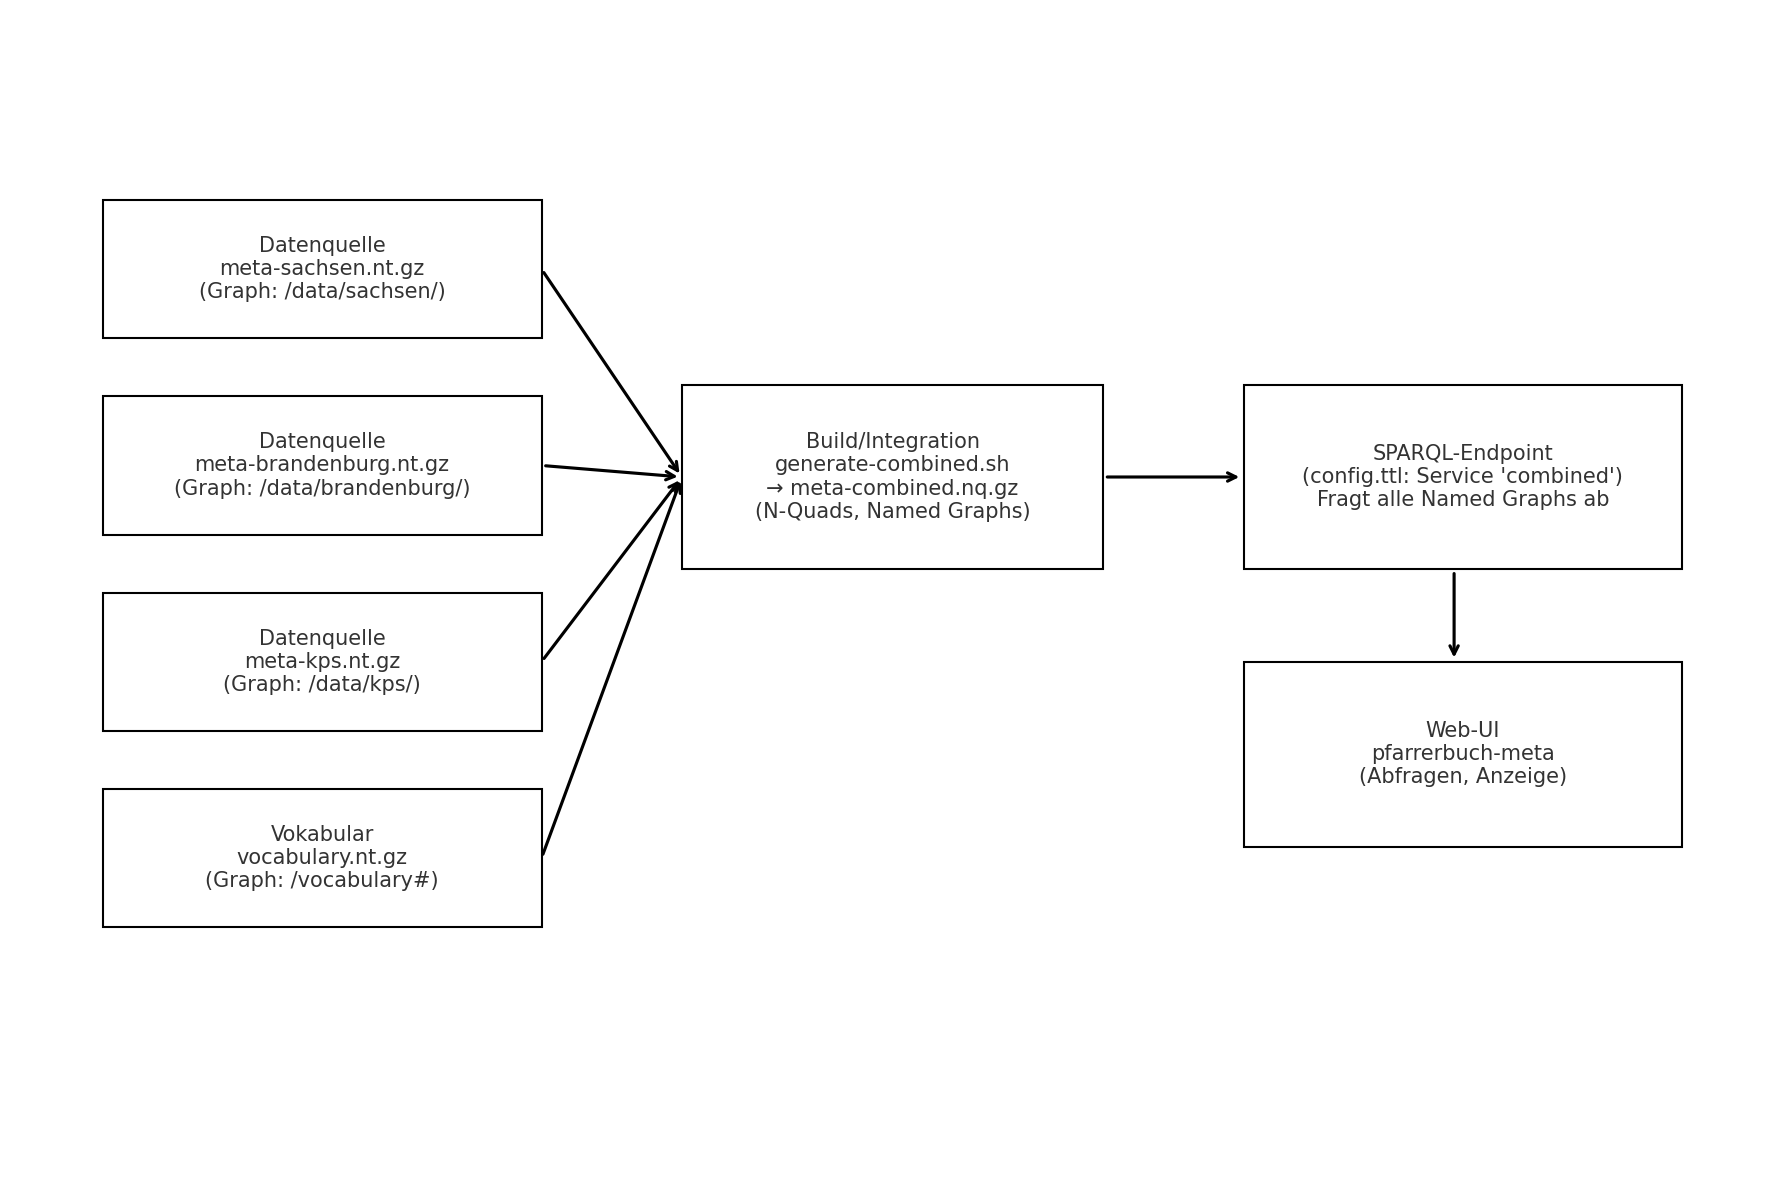
\includegraphics[width=\linewidth]{Abbildungen/Aufbau_Pfarrerdatenbank.jpg}
\caption{Architektur der Pfarrerdatenbank (Quellen $\rightarrow$ Build/Integration $\rightarrow$ kombinierter SPARQL-Dienst $\rightarrow$ Web-UI).}
\label{fig:pfarrer-architektur}
\end{figure}

\noindent Die Abbildung zeigt die vier Bausteine: (1) regionale N-Triples und Vokabular, (2) Skriptbasierter Merge nach N-Quads
(\texttt{meta-combined.nq.gz}) mit benannten Graphen, (3) SPARQL-Endpoint \emph{combined} aus \texttt{config.ttl}, (4) die Web-UI.

\subsection{SPARQL-Beispiele (kompakt)}
\noindent Präfixe (für alle Beispiele):
\begin{verbatim}
PREFIX pfb: http://meta-pfarrerbuch.evangelische-archive.de/vocabulary#

PREFIX rdf: http://www.w3.org/1999/02/22-rdf-syntax-ns#

PREFIX rdfs:http://www.w3.org/2000/01/rdf-schema#

PREFIX xsd: http://www.w3.org/2001/XMLSchema#

\end{verbatim}

\paragraph{(a) Anzahl Personen gesamt und pro Graph}
\begin{verbatim}
SELECT (COUNT(DISTINCT ?p) AS ?personenGesamt) WHERE {
?p rdf:type pfb:Person .
}

SELECT ?g (COUNT(DISTINCT ?p) AS ?anzahl) WHERE {
GRAPH ?g { ?p rdf:type pfb:Person . }
} GROUP BY ?g
\end{verbatim}

\paragraph{(b) Personen mit Name und Geburtsjahr}
\begin{verbatim}
SELECT ?p ?nach ?vor ?jahr WHERE {
?p rdf:type pfb:Person ;
pfb:nachname ?nach ;
pfb:vorname ?vor ;
pfb:hatLebensabschnitt ?la .
?la rdf:type pfb:Geburt .
OPTIONAL { ?la pfb:jahr ?jahr }
} LIMIT 50
\end{verbatim}

\paragraph{(c) Auf Sachsen eingrenzen (benannter Graph)}
\begin{verbatim}
SELECT ?p ?nach ?vor WHERE {
GRAPH http://meta-pfarrerbuch.evangelische-archive.de/data/graphs/sachsen
 {
?p rdf:type pfb:Person ;
pfb:nachname ?nach ;
pfb:vorname ?vor .
}
} LIMIT 50
\end{verbatim}

\paragraph{(d) Geburtsort (sofern vorhanden)}
\begin{verbatim}
SELECT ?p ?nach ?vor ?ort WHERE {
?p rdf:type pfb:Person ;
pfb:nachname ?nach ;
pfb:vorname ?vor ;
pfb:hatLebensabschnitt ?la .
?la rdf:type pfb:Geburt .
OPTIONAL { ?la pfb:hatOrt ?ort }
} LIMIT 50
\end{verbatim}

\subsection{Hinweise zur Nutzung und Qualität}
Für explorative Analysen empfiehlt sich, Ergebnisse zunächst pro benanntem Graph zu betrachten, um regionale Modellierungsdetails zu erkennen. Provenienzangaben (\texttt{pfb:derivedFrom}) können für Nachprüfbarkeit herangezogen werden. Eine formale Datenprüfung via SHACL ist im gelieferten Material nicht enthalten; das Modell ist jedoch dafür ausgelegt (z.,B. Kardinalitäten für \texttt{pfb:vorname}/\texttt{pfb:nachname}, Typbeschränkungen für \texttt{pfb:jahr}/\texttt{xsd:integer} etc.) und kann bei Bedarf ergänzt werden.

\subsection{Fazit}
Die Pfarrerdatenbank stellt einen integrierten RDF-Wissensgraph über mehrere Regionen bereit. Das eigene Vokabular und die klare Trennung per benannten Graphen ermöglichen sowohl aggregierte Queries als auch präzise Regionalsichten. Über den kombinierten SPARQL-Endpunkt versorgt die Web-UI Forschende und die interessierte Öffentlichkeit mit konsistenten, zitierfähigen Daten.








\section{Einführung in Large Language Models}
\label{sec:llm}

\subsection{Einordnung und Motivation}
Große Sprachmodelle (Large Language Models, LLMs) sind neuronale Netze, die auf umfangreichen Textkorpora mit einem Sprachmodellierungsziel vortrainiert werden und anschließend durch Prompting, ggf.\ Feintuning und Ausrichtungstechniken (z.\,B.\ RLHF) eine breite Palette von Sprachaufgaben bearbeiten.\footnote{Ein einführender Überblick findet sich u.\,a.\ in \cite{campesatoLLMIntro}.} 
Zentrale Triebfeder ihrer Leistungsfähigkeit ist die \emph{Transformer}-Architektur \cite{vaswani2017attention} in Kombination mit (i) Skalierung der Modell-, Daten- und Rechenbudgets, (ii) effektiven Prompting-Methoden zur Nutzung von In-Context-Lernen \cite{brown2020language,wei2022chain}, (iii) \emph{Tool\-Use} durch externe Aktionen \cite{yao2023react} sowie (iv) Ausrichtung an menschlicher Intention mittels \emph{Instruction Tuning} und \emph{RLHF} \cite{ouyang2022training}. 
Dieses Kapitel führt die notwendigen Grundlagen zusammen und stellt Verbindungen zu Sicherheit, Datenschutz und Retrieval-Erweiterungen her \cite{abadi2016deep,carlini2021extracting,lewis2020rag}. 

\paragraph{Ziele des Kapitels.}
Wir geben (1) eine architektonische und algorithmische Basis, (2) ein konsolidiertes Bild der Kernparadigmen (In-Context-Lernen, CoT, ReAct, RLHF), (3) einen Überblick über Daten-/Decoding-Fragen (Degeneration, Halluzination), (4) Bausteine für wissensintensive Aufgaben (RAG, KG-QA via LC-QuAD~2.0 \cite{dubey2019lcquad2}) und (5) Implikationen für Sicherheit und Datenschutz (Differential Privacy; Extraktionsangriffe). 

\subsection{Transformer‐Grundlagen}
\subsubsection{Aufmerksamkeitsmechanismus}
Der Transformer \cite{vaswani2017attention} ersetzt rekurrente/konvolutionale Netze durch \emph{Self-Attention}. Für Token-Repräsentationen $X \in \mathbb{R}^{n \times d}$ werden \emph{Queries}, \emph{Keys}, \emph{Values} berechnet: $Q=XW_Q$, $K=XW_K$, $V=XW_V$. Die Aufmerksamkeitsausgabe lautet
\[
\mathrm{Attention}(Q,K,V)= \mathrm{softmax}\!\left(\frac{QK^\top}{\sqrt{d_k}}\right) V.
\]
\emph{Multi-Head Attention} projiziert in $h$ Untermengen, um verschiedene Beziehungsarten parallel zu modellieren. Positionsinformationen werden über (sinusoidale oder gelernte) \emph{Positional Encodings} injiziert. 

\subsubsection{Encoder–Decoder vs.\ Decoder-only}
Encoder–Decoder-Modelle (z.\,B.\ T5) eignen sich für Seq2Seq-Aufgaben; \emph{Decoder-only} (GPT-Familie) modellieren $p(x_t\mid x_{<t})$ und sind für generatives Prompting weit verbreitet \cite{brown2020language}. Die Rechenkomplexität der dichten Attention ist $\mathcal{O}(n^2)$; Varianten mit lokaler/sparscher Attention reduzieren dies in langen Kontexten.

\subsubsection{Vortraining: Ziel, Tokenisierung, Daten}
Standard ist \emph{Causal Language Modeling} (CLM) mit Byte-Pair/Unigram-Tokenisierung. Große Webkorpora (Common Crawl, WebText, Bücher, Wikipedia) werden gefiltert und \emph{dedupliziert}, um Qualität zu erhöhen und Leaks in Val/Test zu mindern \cite{brown2020language}. 

\subsection{Dekodierung und Textqualität}
\subsection{Greedy vs.\ stochastische Verfahren}
Greedy/Beam erzeugen oft wiederholungsreiche, „zu wahrscheinliche“ Texte. Stochastische Verfahren wie \emph{Top-$k$} und \emph{Nucleus Sampling} ($p$-Sampling) verbessern Varianz. 

\subsubsection{Neural Text Degeneration}
Holtzman et al.\ zeigen, dass die Maximierung der sequenziellen Likelihood zu \emph{Degeneration} (Wiederholungen, Langeweile) führen kann und plädieren für kalibriertes Sampling (\emph{nucleus}) \cite{holtzman2020curious}. Für Qualitätskontrolle sind Wiederholungs-Penalities und Länge/Stopkriterien wichtig. 

\subsection{Skalierung und In-Context-Lernen}
\subsubsection{GPT-3 als Katalysator}
Brown et~al.\ \cite{brown2020language} trainieren GPT-3 (175B) und evaluieren \emph{Zero/One/Few-Shot} ausschließlich per Prompting ohne Gradientenupdates \cite{brown2020language}. Kernergebnis: Leistungszuwachs mit Modellgröße und Zahl der In-Context-Beispiele; starke Ergebnisse u.\,a.\ in Übersetzung/QA, aber Schwächen bei ANLI/RACE und „Commonsense-Physik“. Die Arbeit diskutiert \emph{Datenkontamination} und evaluiert deren Einfluss. 

\subsubsection{Prompting-Muster}
In der Praxis haben sich etablierte Muster bewährt:
\begin{itemize}
  \item \textbf{Instruktions-Prompting}: präzise Aufgabenformulierung, Formatvorgaben.
  \item \textbf{Few-Shot-Beispiele}: 3–10 prägnante Demonstrationen im Ziel-Format.
  \item \textbf{Rollen/Constraints}: Stil, Länge, Verweise, „Gedanken erst, dann Antwort“.
\end{itemize}
\noindent Beispiel (schematisch):
\begin{verbatim}
Aufgabe: Beantworte Fragen kurz mit Quelle.
Beispiel 1:
  Frage: ...
  Antwort: ... [Quelle: ...]
...
Neue Frage: ...
\end{verbatim}

\subsection{Kettenbasiertes Denken (Chain-of-Thought, CoT)}
CoT ergänzt Beispiele um \emph{Zwischenschritte} (Rationale) und kann mehrschrittiges Denken „freischalten“ \cite{wei2022chain}. 
Wichtige Beobachtungen: (i) Gewinne steigen mit Modellgröße (\emph{emergent}), (ii) \emph{Self-Consistency} (mehrere Stichproben, Mehrheitsentscheid) erhöht Robustheit, (iii) rein „mehr Token“ erklärt die Effekte nicht — die sprachliche Zerlegung ist der Hebel.

\paragraph{Beispiel-Schablone.}
\begin{verbatim}
Frage: ...
Gedanken: Schritt 1: ...; Schritt 2: ...; ...
Antwort: ...
\end{verbatim}

\paragraph{Grenzen.} CoT kann fehlleiten (halluzinierende Begründungen), skaliert schwächer bei kleinen Modellen und ist sensibel gegenüber Prompt-Formulierungen.

\subsection{Reason \& Act: Tool-Nutzung mit ReAct}
ReAct verschachtelt \emph{Thought–Action–Observation} und verbindet sprachliches Denken mit Aktionen (z.\,B.\ Suche/Lookup) \cite{yao2023react}. 
Das reduziert Halluzination, erhöht Nachvollziehbarkeit und schlägt auf wissensintensiven Aufgaben reine Action- oder reine CoT-Baselines.

\paragraph{Muster.}
\begin{verbatim}
Q: ...
Thought 1: Ich sollte X nachschlagen.
Action 1: Search[X]
Observation 1: ...
Thought 2: ...
Action 2: Lookup["..."]
...
Final Answer: ...
\end{verbatim}

\paragraph{Typische Fehlermodi.} Uninformative Suchen, Gedankenschleifen; begrenzte Schrittzahl, besseres Retrieval und Heuristiken (Fallback auf CoT-Self-Consistency) helfen.

\subsection{Instruction Tuning und RLHF}
\subsubsection{Pipeline}
Ouyang et~al.\ \cite{ouyang2022training} zeigen, dass \emph{Instruction-Modelle} via \emph{SFT} (Demonstrationen), \emph{Belohnungsmodell} (Präferenzranking) und \emph{PPO} (mit KL-Regularisierung) von Menschen systematisch bevorzugt werden — teils übertreffen 1{,}3B-Modelle ein 175B GPT-3 \cite{ouyang2022training}. 

\begin{enumerate}
  \item \textbf{SFT}: überwachte Feinanpassung auf Instruktions-Demos.
  \item \textbf{Reward Modeling}: Labele Präferenzen $\Rightarrow$ Skalarbewertung.
  \item \textbf{RL (PPO)}: Optimierung gegen Reward; KL zur SFT-Policy begrenzt Drift.
\end{enumerate}

\paragraph{Befunde.} Mehr Hilfsbereitschaft/Wahrhaftigkeit, geringere Toxizität (unter „respektvollen“ Prompts), und geringere \emph{Alignment Tax} durch Mischen mit Pretrain-Updates (PPO-PTX). Bias/Halluzination bleiben Forschungsfelder.

\subsection{Wissensintensive Aufgaben: Retrieval-Augmented Generation}
\subsubsection{Prinzip}
RAG trennt parametrisierte Weltkenntnis (LM) und nicht-parametrisches Wissen (\emph{Index}) \cite{lewis2020rag}. Pipeline: (1) Query-Formulierung, (2) Retriever (BM25/DPR/ColBERT), (3) Aggregation der Evidenz (Late/Joint Fusion), (4) Generator konditioniert auf Belege. 
Vorteile: aktuellere Fakten, Transparenz, geringere Halluzination, besseres \emph{Attribution}. 

\subsubsection{KG-QA und LC-QuAD 2.0}
Für \emph{Knowledge Graph QA} koppeln Modelle Retrieval/Reasoning mit SPARQL-Ableitung; LC-QuAD~2.0 bietet komplexe, mehrhopfige KG-Fragen über Wikidata/DBpedia \cite{dubey2019lcquad2}. Prompting kann \emph{Schema-Ahnung} (Entitäten/Relationen) fördern; alternativ generieren Modelle erst \emph{Zwischenformate} (z.\,B.\ NL2Logic) und führen dann Abfragen aus.

\subsection{Strukturiertes Ausgeben}
LLMs sind „free-form“ — viele Anwendungen verlangen jedoch \emph{strukturierte} Ausgaben (JSON, Tabellen, SQL, SPARQL). Optionen:
\begin{itemize}
  \item \textbf{Constrained Decoding}: Grammatik/Regex/JSON-Schema zur Laufzeit erzwingen.
  \item \textbf{Schema-Prompting}: strikte Beispiele/Validierungs-Hinweise.
  \item \textbf{RL nach Schema-Belohnung}: Belohnt valide und semantisch korrekte Strukturen (vgl.\ \cite{cong2023schema}).
\end{itemize}

\subsection{Sicherheit, Datenschutz und verantwortungsvolle Nutzung}
\subsubsection{Extraktion von Trainingsdaten}
Arbeiten wie \cite{carlini2021extracting} zeigen, dass Modelle memorisierte Trainingsfragmente \emph{extrahierbar} machen können (z.\,B.\ seltene Sequenzen, PII). Risikofaktoren: Overfitting, Deduplikationsfehler, aggressive Sampling-Einstellungen.

\subsubsection{Differential Privacy (DP)}
DP-SGD \cite{abadi2016deep} begrenzt den Beitrag einzelner Beispiele durch Gradientenclipping + Rauschen und liefert formale Garantien ($\varepsilon,\delta$). Trade-off: Genauigkeit vs.\ Privatsphäre; praktikabel vor allem in kleineren/feinabgestimmten Settings oder beim Training von \emph{Retrievern}/Hilfsmodellen.

\subsubsection{Halluzination und Attribution}
Halluzinationen entstehen u.\,a.\ durch fehlende Evidenz und glatte LM-Priors. Gegenmaßnahmen: RAG/Tool-Use (ReAct), Quellenangaben, Unsicherheitskommunikation, konservative Dekodierung, Post-Verifikation (z.\,B.\ konsensbasierte Selbstprüfung).

\subsection{Evaluierung}
\subsubsection{Automatisch vs.\ menschlich}
Perplexity ist nur ein Vorindikator. Aufgabenmetriken (EM/F1/ROUGE/Accuracy) und menschliche Präferenzbewertungen (Hilfsbereitschaft, Wahrhaftigkeit, Harmlosigkeit) sind komplementär \cite{ouyang2022training}. 

\subsubsection{Reasoning-Spezifika}
Für CoT/Tool-Use sollten \emph{Rationale} und \emph{Trajektorien} mitbewertet werden (Korrektheit, Konsistenz, Zitierbarkeit). Selbstkonsistenz und Stresstests (Distraktoren, Gegenfakten) erhöhen Aussagekraft.

\subsection{Grenzen und offene Herausforderungen}
\begin{itemize}
  \item \textbf{Skalierungskosten \& Effizienz}: Speicher/Inference; Sparsity (MoE), KV-Caching, distillation.
  \item \textbf{Kontextlänge}: Quadratische Attention vs.\ Long-Context-Methoden; Retrieval als Entlastung.
  \item \textbf{Robustheit/Bias}: Datenkurationslücken, gesellschaftliche Auswirkungen; Evaluationslücken.
  \item \textbf{Erklärbarkeit}: Rationale $\neq$ wahre interne Begründung; dennoch nützlich zur Auditierbarkeit.
\end{itemize}

\subsection{Praxisbausteine (Kochrezepte)}
\subsubsection*{Prompting (Zero/Few-Shot)}
\begin{verbatim}
Rolle: Du bist ein präziser Assistent.
Aufgabe: Beantworte die Frage in 2-3 Sätzen mit Quelle.
Format: Antwort + [Quelle: URL/Titel].

Beispiele:
Q: ...
A: ... [Quelle: ...]

Neue Frage: ...
\end{verbatim}

\subsubsection*{CoT + Self-Consistency}
\begin{verbatim}
Anweisung: Denke Schritt-für-Schritt. Gib am Ende NUR "Antwort: <...>" aus.
(Bei Deployment 5-10 Stichproben generieren, Mehrheitsvotum.)
\end{verbatim}

\subsubsection*{ReAct-Skelett (mit Wikipedia-API o. RAG)}
\begin{verbatim}
Q: ...
Thought 1: ...
Action 1: Search[...]
Observation 1: ...
Thought 2: ...
Action 2: Lookup["..."]
Final Answer: ...
\end{verbatim}

\subsubsection*{Strukturierte Ausgabe (JSON-Template)}
\begin{verbatim}
Gib ausschließlich validen JSON im folgenden Schema aus:
{"answer": "<string>", "evidence": [{"title": "...", "url": "..."}]}
\end{verbatim}

\subsection{Zusammenfassung}
LLMs kombinieren Transformernetzwerke, skalengetriebenes Vortraining und in-Kontext-Anpassung zu universellen Sprachwerkzeugen. \emph{CoT} verbessert mehrschrittiges Denken, \emph{ReAct} verankert Antworten in externer Evidenz, und \emph{RLHF} richtet Modelle auf menschliche Präferenzen aus. Für wissensintensive Szenarien ist \emph{RAG} ein zentraler Baustein. Sicherheit und Datenschutz erfordern sorgfältige Datenkuration, Evaluationshygiene, Privatsphäre-Techniken und verantwortliches Deployment. 

\subsection*{Weiterführende Literatur}
\begin{itemize}
  \item Transformer und Attention \cite{vaswani2017attention}
  \item GPT-3 und In-Context-Lernen \cite{brown2020language}
  \item Chain-of-Thought \cite{wei2022chain}
  \item ReAct \cite{yao2023react}
  \item RLHF/Instruction Tuning \cite{ouyang2022training}
  \item RAG \cite{lewis2020rag}
  \item Neural Text Degeneration \cite{holtzman2020curious}
  \item Differential Privacy \cite{abadi2016deep}
  \item Data Extraction \cite{carlini2021extracting}
  \item LC-QuAD~2.0 \cite{dubey2019lcquad2}
  \item Schema-basiertes RL für strukturierte Outputs \cite{cong2023schema}
\end{itemize}






\section{Prompt-Programmierung und Few-Shot Learning}
\label{sec:prompting}


\subsection{Von \emph{Pre-Train, Fine-Tune} zu \emph{Pre-Train, Prompt, Predict}}
In der aktuellen Entwicklung der Sprachverarbeitung hat sich das Paradigma von rein aufgaben\-spezifischer Supervision hin zu vortrainierten Sprachmodellen (LMs) mit Aufgabenspezifikation über Prompts verschoben. Während klassische Systeme die bedingte Wahrscheinlichkeit \(P(y \mid x;\theta)\) direkt durch überwachten Lernens optimieren, modellieren Prompting-Methoden die Textwahrscheinlichkeit \(P(x;\theta)\) und reformulieren Aufgaben so, dass ein LM mit geeigneter Texteingabe (\emph{Prompt}) die gewünschte Ausgabe produziert \cite{liu2023survey}. Dieses \emph{Pre-Train, Prompt, Predict}-Denken bietet drei zentrale Vorteile: (i) Nutzung großskaliger Rohtexte für das Vortraining, (ii) wenige bis keine gelabelten Daten (\emph{few-/zero-shot}) durch geschickte Aufgabenformulierung, (iii) schnelle Adaptierbarkeit über Prompt- statt Objektiv-Engineering \cite{liu2023survey}.

\subsection{Bausteine des Promptings}
\subsubsection{Prompt-Template-Engineering}
Die Wahl der Prompt-Form prägt maßgeblich die Modellleistung. Gängige Formen sind (i) \emph{Prefix}-Prompts (auto\-regressive LMs; generative Aufgaben), (ii) \emph{Cloze}-Prompts (maskierte LMs; Lückentext), (iii) Vorlagen für Mehrfacheingaben (z.\,B. Satzpaare) \cite{liu2023survey}. Template-Design kann \emph{manuell} (intuitiv, aber fehleranfällig) oder \emph{automatisiert} erfolgen:
\begin{itemize}
  \item \textbf{Diskrete Prompts}: Mining aus Korpora, Paraphrasierung, gradientenbasierte Suche, generative Template-Erzeugung mit seq2seq-LMs; statisch oder dynamisch pro Eingabe \cite{liu2023survey}.
  \item \textbf{Kontinuierliche (``soft'') Prompts}: Optimierung von Prompt-Embeddings (z.\,B. Prefix-/Prompt-Tuning), teils initiiert durch diskrete Seeds oder als Hybrid mit harten Tokens \cite{liu2023survey}.
\end{itemize}

\subsubsection{Prompt-Answer-Engineering}
Neben der Vorlage ist auch der \emph{Antwortraum} entscheidend: Token, Spannen oder ganze Sätze. Für Klassifikation sind häufig eingeschränkte Labelwörter (\emph{Verbalizer}) mit Mapping auf Klassen sinnvoll; für Generierung werden längere Sequenzen verwendet. Analog zum Template lassen sich auch Antwortmengen manuell definieren, paraphrasieren, heuristisch durchsuchen oder kontinuierlich optimieren \cite{liu2023survey}.

\subsubsection{Mehrfach-Prompts und Kontext}
Leistung und Stabilität steigen oft durch \emph{Prompt-Ensembling} (gleich-/gewichtete Mittelung, Mehrheitsvotum, Distillation) sowie \emph{Prompt-Augmentation} über \emph{In-Context}-Demonstrationen (Beispielauswahl, -reihenfolge, Retrieval)\cite{liu2023survey}. Für komplexe Aufgaben helfen \emph{Komposition} (Unterprompts komponieren) und \emph{Dekomposition} (Problem in Teilprompts zerlegen), um Struktur sichtbar zu machen \cite{liu2023survey}.

\subsection{Trainingsstrategien im Prompting-Spektrum}
Prompting kann rein \emph{tuning-frei} (reines Prompting, ggf. mit Demonstrationen) oder mit Parameterupdates betrieben werden:
\begin{enumerate}
  \item \textbf{Tuning-frei}: Zero-/Few-Shot ohne LM-Update; maximal effizient, aber prompt-sensitiv \cite{liu2023survey}.
  \item \textbf{Fixiertes LM \& Prompt-Tuning}: Nur Prompt-Parameter werden gelernt (z.\,B. Prefix-/Prompt-Tuning); meist robust im Few-Shot, begrenzte Kapazität bei viel Daten \cite{liu2023survey}.
  \item \textbf{Fixiertes Prompt \& LM-Tuning}: Klassisches Fine-Tuning mit fester Vorlage; oft starker Few-Shot-Booster \cite{liu2023survey}.
  \item \textbf{Prompt+LM-Tuning}: Gemeinsame Optimierung; flexibel und stark, aber ressourcenintensiv \cite{liu2023survey}.
\end{enumerate}

\subsection{Argumentation mit \emph{Chain-of-Thought} und \emph{Self-Consistency}}
\subsubsection{Chain-of-Thought (CoT)}
CoT-Prompting erweitert Few-Shot-Beispiele um natürliche Zwischenschritte (\emph{Reasoning-Rationale}). Große Modelle (typisch \(\ge\)100B Parameter) zeigen damit emergente Denkfähigkeiten: Sie zerlegen Aufgaben in interpretierbare Teilrechnungen und steigern die Genauigkeit besonders bei mehrstufigen mathematischen, logischen und symbolischen Benchmarks \cite{wei2022cot}. CoT ist promptbasiert (kein zusätzliches Training), verbessert Nachvollziehbarkeit und Fehleranalyse und wirkt besonders bei komplexen Aufgaben.

\subsubsection{Self-Consistency}
Anstelle einer einzelnen gierigen CoT-Generierung wird bei \emph{Self-Consistency} ein diverser Satz an Denkpfaden gesampelt und anschließend die \emph{konsistenteste} Endantwort via Mehrheitsvotum (oder gewichteter Marginalisierung) gewählt. Diese \emph{sample-and-marginalize}-Strategie verbessert CoT über viele Benchmarks signifikant (z.\,B. GSM8K, SVAMP, ARC, StrategyQA) und ist trainingsfrei sowie modellagnostisch \cite{wang2022selfconsistency}. Praktisch zeigt sich eine schnelle Sättigung: Wenige Pfade (z.\,B. 5–10) heben die Leistung stark an.

\subsubsection{Kalibrierung vor der Nutzung}
Few-Shot-Prompting ist oft volatil: Reihenfolgeeffekte, Mehrheitslabel- und Aktualitätsbias sowie Common-Token-Bias verschieben die Ausgabeverteilung. \emph{Kontextuelle Kalibrierung} schätzt zunächst Antworttendenzen auf inhaltsfreien Inputs (z.\,B. ``N/A'') und korrigiert dann die Wahrscheinlichkeiten. Das reduziert Varianz und steigert die mittlere Genauigkeit deutlich, ohne zusätzliche Daten \cite{zhao2021calibrate}. Kalibrierung und CoT/Self-Consistency ergänzen sich in der Praxis.

\subsection{Prompting jenseits klassischer Benchmarks: KGQA \& Text-zu-SPARQL}
\subsubsection{Direktantwort vs. Text-zu-SPARQL}
Für Wissensgraph-Fragen (\emph{KGQA}) zeigen Studien, dass \emph{Text-zu-SPARQL} mit geeigneten Prompts stabiler und genauer ist als direkte Freitextantworten: Das LM übersetzt die NL-Frage in SPARQL, die Ausführung liefert belastbare Resultate. Besonders effektiv ist die Kombination aus T-Box (Schema) und A-Box (Instanzen) sowie die Reduktion des dem LM übergebenen Graphausschnitts (\emph{Fragmentierung}) \cite{avila2024autokgqagpt}. Das Framework \emph{Auto-KGQAGPT} illustriert:
\begin{itemize}
  \item Offline-Indizierung von Klassen/Eigenschaften/Instanzen,
  \item Online-Selektion relevanter Teilgraphen pro Frage,
  \item Generierung mehrerer SPARQL-Varianten und Wahl der bestpassenden anhand Ausführungsergebnissen,
  \item Erzeugung der finalen NL-Antwort aus Query+Result.
\end{itemize}
Ergebnisse zeigen: weniger Tokens, weniger Halluzinationen, robuste Genauigkeit—insbesondere bei arithmetischen/aggregativen Anfragen, bei denen direkte Generierung häufiger fehlgeht \cite{avila2024autokgqagpt}.

\subsubsection{Praktische Implikationen}
Für reale KGs (hohe Kardinalitäten, Inferenz-Tripel) ist \emph{Fragmentierung} technisch essenziell (Kontextfenster), fachlich hilfreich (Relevanzfokus) und methodisch robust (SPARQL als \emph{Exekutionsgrund}). Prompt-Templates sollten Präfixe/Namespaces sichern, optionale Properties als \texttt{OPTIONAL} behandeln und Zeichenkettenfilter konsistent (\texttt{regex}, \texttt{i}-Flag) spezifizieren \cite{avila2024autokgqagpt}.

\subsection{Von Prompt-Ketten zu selbstverbessernden Pipelines: DSPy}
\emph{DSPy} abstrahiert LM-Aufrufe als deklarative, parametrisierte Module (\emph{Signaturen, Module, Teleprompter}) und kompiliert ganze Pipelines automatisch zu hochwertigen Prompt-/Finetuning-Strategien \cite{khattab2023dspy}. Kerngedanke:
\begin{itemize}
  \item \textbf{Signaturen} beschreiben \emph{was} transformiert werden soll (z.\,B. Frage\(\rightarrow\)Antwort), nicht \emph{wie} ein Prompt zu formulieren ist.
  \item \textbf{Module} (z.\,B. \texttt{Predict}, \texttt{ChainOfThought}, \texttt{ReAct}) kapseln Techniken und sind austauschbar.
  \item \textbf{Teleprompter (Compiler)} bootstrappen wenige, aber nützliche Demonstrationen, wählen Hyperparameter (z.\,B. per Random/Search/Optuna) und können feintunen, ensemblel'n oder Kontrollfluss variieren.
\end{itemize}
Fallstudien zeigen, dass wenige Zeilen DSPy-Code Pipelines erzeugen, die handgetunte Prompt-Ketten \emph{ohne} manuell kuratierte Prompts übertreffen, und dies auch mit kleineren offenen LMs wettbewerbsfähig leisten \cite{khattab2023dspy}. Für die Praxis bedeutet dies: weniger fragile String-Prompts, mehr reproduzierbare, automatisch verbesserbare Komponenten—ideal für komplexe Aufgaben wie Multi-Hop-Retrieval, KGQA oder Agent-Loops.

\subsection{Offene Herausforderungen und Best Practices}
\subsubsection*{Offene Punkte}
\begin{itemize}
  \item \textbf{Modellwahl \& Transfer}: Prompts generalisieren nicht immer über Modellgrößen/-familien hinweg; systematische Vergleiche fehlen \cite{liu2023survey}.
  \item \textbf{Skalierbarkeit}: Ensemble/CoT/Self-Consistency kosten Zeit/Compute; adaptive Budgetierung (z.\,B. nur auf schwierigen Instanzen) ist ein aktives Feld.
  \item \textbf{Kalibrierung \& Bias}: Kontextkalibrierung hilft, doch bleibt Prompt-Design anfällig für Formateffekte \cite{zhao2021calibrate}.
  \item \textbf{Struktur}: Tabellen/Graphen/Pläne elegant in Templates/Antworten zu gießen, ist weiterhin herausfordernd \cite{liu2023survey}.
\end{itemize}

\subsubsection*{Best Practices (konkret umsetzbar)}
\begin{enumerate}
  \item \textbf{Start} mit klarer Aufgabenformulierung \(\rightarrow\) geeignete Promptform (Prefix/Cloze) und kleiner, kuratierter Antwortraum.
  \item \textbf{Stabilität} durch \emph{Prompt-Augmentation} (repräsentative Demonstrationen) und \emph{Kontextuelle Kalibrierung} \cite{zhao2021calibrate}.
  \item \textbf{Denkaufgaben}: \emph{CoT} aktivieren; bei Bedarf \emph{Self-Consistency} (5–10 Reasoning-Samples) \cite{wei2022cot,wang2022selfconsistency}.
  \item \textbf{Wissensfragen}: strukturierte Exekution (z.\,B. SPARQL) statt reine Generierung; KG-Fragmentierung plus Vorlagen-Disziplin \cite{avila2024autokgqagpt}.
  \item \textbf{Pipelines}: deklarativ (DSPy) bauen und vom Compiler Demonstrationen/Hyperparameter optimieren lassen \cite{khattab2023dspy}.
  \item \textbf{Evaluation}: Neben Genauigkeit Varianz und Reproduzierbarkeit messen (verschiedene Seeds, Reihenfolgen, Prompt-Formate).
\end{enumerate}

\subsection{Fazit}
Prompting verschiebt den Schwerpunkt von datenintensiver Supervision zu geschickter Aufgabenformulierung. Mit Template- und Answer-Engineering, CoT und Self-Consistency sowie kontextueller Kalibrierung lassen sich starke, robuste Systeme bauen. Für wissensintensive Domänen bietet \emph{Text-zu-SPARQL} eine präzise, skalierbare und halluzinationsarme Alternative. Programmiermodelle wie \emph{DSPy} heben Prompting aus der Ebene fragiler Strings auf modulare, kompilierbare Pipelines. Zusammen liefern diese Bausteine einen praktikablen Werkzeugkasten, um moderne LMs verlässlich, effizient und nachvollziehbar in realen Anwendungen einzusetzen \cite{liu2023survey,wei2022cot,wang2022selfconsistency,zhao2021calibrate,avila2024autokgqagpt,khattab2023dspy}.
Ontologiefragmente werden gezielt gefiltert, um den LLM-Kontext kompakt und relevant zu halten \cite{avila2024autokgqagpt}.





\section{Query-Validierung und Explainability im RDF/SPARQL-Stack}
\label{chap:Query-validation-explainability}

\subsection{Motivation}
RDF, RDFS und OWL beschreiben vorrangig \emph{Struktur}. Für belastbare Datenprodukte brauchen wir zusätzlich:
(i) \textbf{Validierung} gegen modellierte Erwartungen (Constraints),
(ii) \textbf{Erklärbarkeit} von Ergebnissen und Fehlstellen (Provenienz \& Why-Not),
(iii) \textbf{robuste OPTIONAL-Nutzung} für Teilantworten ohne unkontrollierbare Komplexität.
Dieses Kapitel führt drei Bausteine zusammen: SPIN für modellnahe Validierung und Regeln \cite{spin-w3c}, schwach gut konzipiertes (wwd) SPARQL zur sicheren OPT-Verwendung \cite{kaminski-kostylev-beyond-well-designed} und Provenienz-Halbringe als algebraisches Fundament für Explainability \cite{green-provenance-semirings,herschel-why-why-not,herschel-survey}.

\subsection{Validierung mit SPIN}
\subsubsection{Grundidee}
SPIN (\emph{SPARQL Inferencing Notation}) repräsentiert SPARQL als RDF und verknüpft Abfragen direkt mit Klassen:
\begin{itemize}
  \item \texttt{spin:constraint}: Bedingungen (ASK/CONSTRUCT), die Instanzen erfüllen müssen.
  \item \texttt{spin:rule}: Inferenz (CONSTRUCT / UPDATE) zur Ableitung zusätzlicher Tripel.
  \item \texttt{spin:constructor}: Initialwerte beim Anlegen neuer Instanzen.
\end{itemize}
Abfragen laufen im Klassenkontext mit vorgebundener Variable \texttt{?this}; Vererbung erfolgt entlang \texttt{rdfs:subClassOf}. Zur Optimierung kann \texttt{spin:thisUnbound} auf \texttt{true} gesetzt werden, wenn die WHERE-Bedingungen \texttt{?this} selbst binden \cite{spin-w3c}.

\subsubsection{Fehlermeldungen und Auto-Fixes}
CONSTRUCT-Constraints können \texttt{spin:ConstraintViolation} erzeugen (lesbares \texttt{rdfs:label}, \texttt{spin:violationRoot}, \texttt{spin:violationPath}) und \texttt{spin:fix}-Hinweise auf \texttt{spin:UpdateTemplate}s liefern.

\subsubsection{Minimalbeispiel (Constraint)}
\begin{lstlisting}[language=turtle,basicstyle=\ttfamily\small,caption={SPIN-Constraint: Quadrat konsistent halten},label={lst:spin-constraint}]
@prefix ex:   <http://example.org/> .
@prefix rdfs: <http://www.w3.org/2000/01/rdf-schema#> .
@prefix spin: <http://spinrdf.org/spin#> .
@prefix sp:   <http://spinrdf.org/sp#> .

ex:Square a rdfs:Class ;
  spin:constraint [
    a sp:Ask ;
    sp:text """ASK {
      ?this ex:width ?w ; ex:height ?h .
      FILTER(?w != ?h)  # TRUE => Verletzung
    }""" ;
  ] .
\end{lstlisting}

\paragraph{Praxisleitfaden (kurz).}
\begin{itemize}
  \item Lege Prüfungen als \texttt{ASK} an (schnell) und ergänze bei Bedarf \texttt{CONSTRUCT}-basierte Violations mit \texttt{spin:fix}.
  \item Halte Regeln/Constraints \emph{klassenlokal} und granular; nutze Bibliotheken über dereferenzierbare URIs.
  \item Begrenze UPDATE-Regeln (Iterationslimit, Reihenfolge via \texttt{spin:nextRuleProperty}), um Loops zu vermeiden.
\end{itemize}

\subsection{Explainability: Provenienz und Why-Not}
\subsubsection{Algebraisches Fundament}
Annotiere Tupel mit Elementen eines kommutativen Halbrings \(K\) (\emph{K-Relationen}). Relationale Algebra/Datalog werden homomorph auf Annotationen gehoben \cite{green-provenance-semirings}. Dadurch:
\begin{itemize}
  \item \textbf{How-Provenienz}: Polynome (z.\,B. \(t_1 t_2 + t_1 t_3\)) kodieren \emph{wie} Quellen kombiniert wurden.
  \item \textbf{Why-Provenienz}: Zeugen(-basen) zeigen \emph{welche} Quelltupel genügen.
  \item \textbf{Where-Provenienz}: Positionale Herkunft (Zell-/Attributebene) für Kopierursprünge.
  \item \textbf{Rekursion}: Datalog-Provenienz via formale Potenzreihen und Fixpunkte.
\end{itemize}

\subsubsection{Warum-nicht-Erklärungen (fehlende Antworten)}
Zwei Blickwinkel \cite{herschel-why-why-not,herschel-survey}:
\begin{description}
  \item[Instanzbasiert] (abduktiv): Welche minimalen Tupel/Updates würden das gewünschte Ergebnis erzeugen?
  \item[Abfragebasiert] (operatorzentriert): Welche Operatoren/Prädikate schneiden kompatible Tupel ab?
\end{description}
Hybride Ansätze kombinieren beides (Operator als „Culprit“ \emph{und} minimale Datenänderung).

\paragraph{Operative Empfehlungen.}
\begin{itemize}
  \item Provenienz für Ergebnis-Tupel \emph{materialisieren} oder on-the-fly rekonstruierbar halten (Kosten beachten).
  \item Für Why-Not mindestens \emph{Top-Level-Filter} und verworfene Tripelmuster protokollieren.
  \item Visualisierung: kompakte Summaries statt roher Graphen; Aggregation nach Operator/Quelle.
\end{itemize}

\subsection{OPTIONAL richtig einsetzen: wwd-SPARQL}
OPTIONAL ermöglicht Teilantworten, ist aber in voller Allgemeinheit PSPACE-schwer. Das \emph{gut konzipierte} Fragment (wd) zügelt das, deckt die Praxis aber nur teilweise ab. \textbf{Schwach gut konzipierte} Muster (wwd) \emph{erweitern} wd und behalten coNP-Auswertbarkeit bei \cite{kaminski-kostylev-beyond-well-designed}:
\begin{itemize}
  \item Erlaube Variablen von rechten \texttt{OPT}-Seiten außerhalb des Untermusters nur, wenn deren Auftreten \emph{dominiert} (links) und Filter für solche Variablen nur auf \emph{oberster Ebene} stehen.
  \item Normalform: \emph{OPT-FILTER-Normalform} (OF) und \emph{Constraint Pattern Trees} (CPT) machen Prioritäten explizit.
\end{itemize}
\textbf{Best Practices.}
\begin{enumerate}
  \item Links-assoziieren: \((P_1~\mathrm{OPT}~P_2)~\mathrm{OPT}~P_3\) statt \(P_1~\mathrm{OPT}~(P_2~\mathrm{OPT}~P_3)\).
  \item FILTER, die Variablen aus rechten \texttt{OPT}s referenzieren, \emph{nur} auf oberster Ebene.
  \item Denke in OF/CPT-Strukturen; vermeide (wo möglich) tiefe \texttt{OPT}-Nester.
\end{enumerate}

\subsection{Praktische Pipeline}
\begin{enumerate}
  \item \textbf{Modellieren}: Klassen/Eigenschaften (RDFS/OWL) + SPIN-\texttt{constraint}s (Validierung) + optionale SPIN-\texttt{rule}s (Anreicherung).
  \item \textbf{Validieren früh}: Formulare/ETL prüfen via \texttt{ASK}-Constraints; bei Verstößen \texttt{ConstraintViolation} mit \texttt{spin:fix}.
  \item \textbf{Abfragen robust}: Abfrageentwurf in wwd-Form; OF-Normalisierung als Ziel.
  \item \textbf{Erklären}: How/Why-Provenienz für Ergebnisse; Why-Not für fehlende Tupel (operator- und/oder instanzbasiert).
\end{enumerate}

\subsection{Checkliste}
\begin{itemize}
  \item \emph{Constraint-Abdeckung}: Pflichtfelder, Kardinalitäten, Datentypen, konsistente Rollen.
  \item \emph{OPT-Disziplin}: Keine (Opt-R)-Verschachtelungen; Top-Level-FILTER.
  \item \emph{Explainability-Artefakte}: Provenienzpolynome oder komprimierte Summaries; Protokolle für verworfene Bindungen.
  \item \emph{Governance}: Dereferenzierbare URIs für SPIN-Bibliotheken; Regeliteration begrenzen.
\end{itemize}

\subsection{Grenzen und Ausblick}
SPIN bringt Validierung \emph{ins Modell}, erfordert aber Disziplin (Terminierung, Updates). Wwd erlaubt praxisnahe OPTIONALs bei kontrollierter Komplexität; OF/CPT hilft beim Tuning, kann jedoch im Worst Case wachsen. Provenienz skaliert inhaltlich, aber nicht beliebig speicherseitig; visuelle Summarisierung bleibt ein Schlüsselthema \cite{herschel-survey}. Nächste Schritte: domänenspezifische SPIN-Bibliotheken, (halb-)automatische OF-Normalisierung, eingebettete Why-Not-Erklärung in Triple Stores.







\section{Datenschutz und Anonymisierung in SPARQL-Operationen}
\label{sec:privacy}

Dieses Kapitel behandelt Strategien, Modelle und konkrete Mechanismen, um Datenschutz in SPARQL-basierten Systemen (RDF-Speicher, Linked-Data-APIs, Query-Logs) systematisch umzusetzen. Wir beginnen mit rechtlich-konzeptionellen Grundlagen, leiten daraus Angreifermodelle und Schutzziele ab und entwickeln darauf aufbauend technische Maßnahmen: Zugriffskontrolle für RDF/ SPARQL, Pseudonymisierung, Anonymisierung robuster RDF-Graphen, differentielle Privatsphäre (inkl.\ ihres Einsatzes für SPARQL-Antworten und Query-Logs), k-Anonymität via Mikroaggregation sowie betriebliche Leitlinien für Fuseki/Jena. Die Ausgestaltung folgt den W3C \emph{Data on the Web Best Practices} und dem W3C \emph{Data Privacy Vocabulary}.

\subsection{Grundlagen: Rechtsrahmen und Begriffe}
\textbf{Rechtsmaßstab.} Nach EU-DSGVO ist \emph{Anonymisierung} ein irreversibler Prozess; \emph{Pseudonymisierung} reduziert Identifizierbarkeit, bleibt aber personenbezogen. Der Artikel-29-Arbeitskreis betont drei Prüfsteine: \emph{Singling-out}, \emph{Linkability} und \emph{Inference} (schlussfolgernde Offenlegung). Maßnahmen sind nur dann hinreichend, wenn alle drei Risiken angemessen gemindert werden \cite{Art29WPAnonymisation, enisa2019pseudonymisation}.

\textbf{Privacy-by-Design für Webdaten.} W3C \emph{Privacy Principles} fordern Zweckbindung, Datenminimierung, Sicherheit, Transparenz/ Wahlmöglichkeiten und Verantwortlichkeit \cite{W3CPrivacyPrinciples}. Das W3C \emph{Data Privacy Vocabulary} (DPV) liefert Begriffe zur konsistenten Dokumentation von Zwecken, Rechtsgrundlagen, Empfängern, Speicherfristen u.\,a.\ als Metadaten \cite{W3CDPV}. Veröffentlichungs- und Betriebsprozesse sollen den \emph{Data on the Web Best Practices} folgen (Metadaten, Provenienz, Versionierung, Mehrformatauslieferung, Feedback) \cite{W3CDWBP}.

\subsection{Angreifermodelle und Schutzziele}
\textbf{Angreifer.} (i) Passiv: nutzt offen zugängliche SPARQL-Endpunkte und Dumps; (ii) Aktiv: injiziert Abfragen/ Daten zur späteren Re-Identifikation (Sybil/ Poisoning); (iii) Verknüpfer: kombiniert externe Quellen (Linkage). \textbf{Schutzziele:} (a) Verhindern eindeutiger Re-Identifikationen (\emph{singling-out}), (b) Minimieren von Linkage-Erfolg, (c) Begrenzen von Inferenz über sensible Attribute, (d) Verfügbarkeit und Nützlichkeit der Daten für legitime Zwecke.

\subsection{Zugriffskontrolle als Grundschutz (AuthN/AuthZ)}
\textbf{Serverseitig.} Apache Fuseki unterstützt HTTPS, Benutzer/Passwort (Basic/Digest nur über TLS), ACLs auf Server-, Datensatz-, Endpunkt- und (read-only) Graph-Ebene; der Union-Graph und der Default-Graph sind steuerbar \cite{FusekiAccess}. \textbf{In-Graph-Policies.} \emph{Jena Permissions} kapselt Graph/Model-APIs mittels dynamischer Proxys und erzwingt CRUD-Entscheidungen pro Principal auf Graph- und optional Triple-Ebene via \texttt{SecurityEvaluator} (inkl.\ Caching) \cite{JenaPermissions}. 
\textbf{Designhinweise.} (1) TLS mit vertrauenswürdigen Zertifikaten; (2) Least-Privilege-ACLs; (3) Trennung von \emph{privaten Rohdaten} und \emph{publiken Derivaten}; (4) Audit-Logging.

\subsection{Pseudonymisierung versus Anonymisierung}
\textbf{Pseudonymisierung.} Tokenisierung/Hashing von IDs oder Query-Tokens ist gegen Frequenz- und Kontextangriffe schwach; robustere Varianten benötigen Salts, Schlüsselrotation und Kontext-Verdrillung. \textbf{Anonymisierung.} Für Veröffentlichungen (Dumps, häufige Items) sind formale Verfahren notwendig: differentielle Privatsphäre oder strikte k-Anonymität (mit bekannten Grenzen).

\subsection{Anonymisierung von RDF-Graphen}
\textbf{Strukturelle Risiken.} RDF-Graphen sind über Identifikatoren und Topologie verknüpfbar; Linkage-Angriffe nutzen Hintergrundwissen über Muster, Attributdomänen oder externe Datensätze. Arbeiten zu robusten RDF-Anonymisierungen und den logischen Grundlagen privacy-wahrender Linked-Data-Publikation analysieren, wann Generalisierung/Suppression hinreicht und welche Beschränkungen nötig sind \cite{delanaux-linkage, logical-foundations-lda}. 
\textbf{Praktische Optionen.} (i) Identifier-Generalisierung/ Zufalls-IRIs für lokale Ressourcen; (ii) Attribut-Binning und Hierarchisierung; (iii) Topologie-Vergröberung (Entität zu Typ/ Superklasse); (iv) strikte Provenienz: dokumentiere alle Transformationen (PROV-O).

\subsection{Differential Privacy (DP) für SPARQL}
\subsection{Definitionen}
Ein (randomisierter) Mechanismus $A$ ist $\varepsilon$-DP, wenn für alle benachbarten Datensätze $D,D'$ und Ausgaben $O$ gilt:
\[
\Pr[A(D)=O]\le e^{\varepsilon}\Pr[A(D')=O].
\]
Schwächungen: $(\varepsilon,\delta)$-DP (Ununterscheidbarkeit) sowie \emph{probabilistic DP}, die mit Wahrscheinlichkeit $\ge 1-\delta$ strikte $\varepsilon$-DP garantiert \cite{GoetzZealous}.

\subsubsection{SPARQL-spezifische Aspekte}
SPARQL umfasst Auswahl, Projektion, Joins, Aggregation und Konstruktion. DP ist unmittelbar einsetzbar für aggregierende, monotone Anfragen (\texttt{COUNT}, \texttt{SUM} über gebundene Domänen) mit bekannter globaler Sensitivität; für frei kombinierte \texttt{OPTIONAL}/\texttt{FILTER}-Muster steigen Sensitivität und Analyseaufwand. Arbeiten zu \emph{Differential Privacy and SPARQL} diskutieren fragmentierte Anfragesprachen, Budgetierung und Rauschen (Laplace/Geometrisch) an Antwort- oder Operator-Kanten \cite{builaranda-dp-sparql}. 
\textbf{Praxisleitfaden.} 
(a) \emph{Fragment}: Aggregations-Untermenge mit statisch beschränkter Kardinalität zulassen; 
(b) \emph{Per-User Contribution Capping}: je Benutzer max.\ $m$ Beiträge; 
(c) \emph{Budget}: $\varepsilon$ sitzungsweise; Komposition beachten; 
(d) \emph{Post-Processing}: Negativwerte truncaten, Seltenes filtern.

\subsubsection{DP-Mechanismen für Endpunkte}
\begin{itemize}
  \item \textbf{Antwort-Perturbation}: Addiere Laplace/Geometrisches Rauschen zu \texttt{COUNT}/\texttt{SUM}; reportiere Konfidenzintervalle.
  \item \textbf{Schema-Perturbation}: Verrausche Histogramme (Häufigkeiten von IRIs/ Literalen) und beantworte Anfragen aus diesen Strukturen.
  \item \textbf{Query Auditing/Refusal}: Lehne Anfragen ab, deren geschätzte Sensitivität die Budgetgrenze sprengt.
\end{itemize}

\subsection{Anonymisierung von Query-Logs und häufigen Items}
Strikte $\varepsilon$-DP ist für Such/Query-Logs oft nutzwertarm; k-Anonymität ist gegen \emph{aktive} Angriffe fragil (Injektion von $k\!-\!1$ Ködern). \textbf{ZEALOUS} bietet einen Mittelweg: Beiträge pro Nutzer auf $m$ begrenzen, Vorfilter $\tau$, Laplace-Rauschen, Nachfilter $\tau'$ und Veröffentlichung nur der (verrauschten) häufigen Items. Damit lässt sich $(\varepsilon,\delta)$-\emph{probabilistic DP} und in Varianten $(\varepsilon,\delta)$-Ununterscheidbarkeit erreichen \cite{GoetzZealous}. 
\paragraph{Parameterwahl (Praxis).} Fixiere $\delta$ (z.\,B.\ 0{,}001), wähle $\varepsilon\in[0{,}5,2]$, setze $\tau=\lceil 2m/\varepsilon\rceil$ zur Minimierung von $\tau'$, und wähle $m$ \emph{unterhalb} der durchschnittlichen Nutzerbeiträge (Abdeckung vs.\ Präzision). 
\paragraph{Nutzwertmetriken.} Top\,$J$-Abdeckung (Recall) und L1/KL-Abstand der relativen Häufigkeiten; häufige Items erhalten gute Präzision, seltene werden eliminiert.

\subsection{k-Anonymität mittels Mikroaggregation (User-Level)}
Für nutzerzentrierte Mining-Aufgaben kann Mikroaggregation echte k-Anonymität auf \emph{Benutzer-Ebene} schaffen: Nutzer werden als Query-Bäume durch Distanzmetriken (Zeit, Rang, Domain-Ähnlichkeit, Levenshtein/Hausdorff über Termmengen) geclustert; anschließend ersetzt der Cluster-\emph{Schwerpunkt} die Individualdaten (\emph{Partition} $\Rightarrow$ \emph{Aggregation}). So wird Re-Identifikation auf $1/k$ begrenzt, bei kontrolliertem Informationsverlust \cite{NavarroUserKAnon}. Einschränkung: syntaktisch (keine Begriffsemantik), aktiv angreifbare Konstellationen bleiben möglich (vgl.\ Inferenz/ Linkage).

\subsection{Online-Streaming: Schwellen-Kryptografie für eindeutige Abfragen}
Um den \emph{Long Tail} eindeutiger/ seltener Abfragen online zu entschärfen, kann Secret-Sharing/ Threshold-Kryptografie eingesetzt werden: Abfragen werden in Shares zerlegt und erst ab Schwellwert $t$ (verschiedene Nutzer) rekonstruierbar. Alternative: Sitzungs-Splitting nach Interessensdomänen zur Reduktion rekonstruierbarer Verläufe \cite{AdarQueryLogs}. Diese Mechaniken sind für Streaming-Pipelines nützlich, mindern aber Korrelationen/ Feinkörnigkeit.

\subsection{Betriebsarchitektur für SPARQL mit Datenschutz}
\label{sec:privacy-governance}
\textbf{Schichtenmodell.}
\begin{enumerate}
  \item \emph{Ingest \& Private Zone}: Rohdaten/Logs, Zugriff streng begrenzt (Fuseki ACLs, Jena Permissions).
  \item \emph{Anonymisierungs-Layer}: (i) DP-Antworten für Endpunkt-Aggregation; (ii) ZEALOUS für häufige Items; (iii) Mikroaggregierte Nutzeransichten hinter stärkeren Policies.
  \item \emph{Publikations-Zone}: read-only Datensätze/Graphen, TLS, AuthN, Graph-ACLs; Metadaten mit DCAT, DPV, PROV-O; Bulk-Dump + API.
\end{enumerate}
\textbf{Rate-Limit/ Budget.} Anfrage-Budgetierung pro Principal (DP-Budget $\varepsilon$), Throttling, Captcha/ Bot-Schutz; Ablehnung hochsensitiver Anfragen. 
\textbf{Provenienz und Versionierung.} Jede Veröffentlichung enthält \emph{maschinell} (PROV-O, DQV) dokumentierte Parameter ($\varepsilon,\delta,m,\tau,\tau'$), Datenbasis (Zeit/Scope), Qualität und Lizenz; persistente URIs für „neueste“ vs.\ datierte Version (Memento-fähig) \cite{W3CDWBP}.

\subsection{Leitlinien \& Checkliste}
\begin{itemize}
  \item \textbf{Minimalprinzip:} Daten und Antworten so grob wie möglich, so fein wie nötig.
  \item \textbf{SPARQL-Fragment:} Aggregations-Teilmenge mit statischer Sensitivitätsgrenze; keine Volltext-Lecks (\texttt{STRSTARTS}/\texttt{CONTAINS} nur auf whitelisted Feldern).
  \item \textbf{DP für Aggregation:} Antwort-Rauschen + Budget + Per-User-Capping.
  \item \textbf{Logs:} Für Trendanalysen ZEALOUS; für Nutzer-Clustering Mikroaggregation.
  \item \textbf{Betrieb:} TLS, AuthN, Graph/Triple-Policies, Audit; Abuse-Schutz (Rate-Limits, Retry-Delays).
  \item \textbf{Publikation:} DCAT/DPV/PROV-Metadaten, Lizenz, Version, Bulk+API, Feedbackkanal.
\end{itemize}

\subsection{Grenzen und Forschungslücken}
DP in voll allgemeinem SPARQL (mit optionalen Mustern, Rekursion, Konstruktion) ist offen; robuste RDF-Anonymisierung gegen starke Linkage-Gegner bleibt schwierig. Semantische Ähnlichkeiten (statt reiner Edit-Distanzen) könnten Mikroaggregation verbessern; gleichzeitig erhöht sich der Angriffsraum. Für produktive Endpunkte ist die Kombination aus starkem Grundschutz (AuthN/Z), restriktivem SPARQL-Fragment, DP-Aggregationen und anonymisierten Veröffentlichungen derzeit der praktikable Kompromiss.

\medskip
\noindent\textbf{Kernaussage.} K-Anonymität allein genügt nicht; strikte $\varepsilon$-DP ist oft zu restriktiv. In der Praxis bewährt sich ein \emph{Policy + Mechanism}-Ansatz: starke Zugriffskontrolle, formal begründete Anonymisierung (ZEALOUS/DP) für häufige Items und (wo nötig) k-anonyme Nutzerprofile via Mikroaggregation, flankiert von sauberer Publikations-Governance (W3C-BPs, DPV, PROV).











\chapter{Verwandte Arbeiten}
\label{sec:related-work}

Dieses Kapitel ordnet unseren Beitrag entlang von fünf Strängen ein: (i) \emph{NL{\textrightarrow}SPARQL \& KGQA}, (ii) \emph{visuelle Query-Builder}, (iii) \emph{Anonymisierung \& Differential Privacy für RDF/SPARQL}, (iv) \emph{Zugriffskontrolle für RDF \& Linked Data}, und (v) \emph{Governance-Vokabulare (DPV)}. Über alle Stränge hinweg adressieren wir die Lücke zwischen nutzerfreundlicher Anfrageerstellung, formaler Datenschutzsicherung und durchsetzbarer Richtlinienprüfung vor der SPARQL-Ausführung.

\subsection{NL{\textrightarrow}SPARQL und Fragebeantwortung auf Wissensgraphen}
Frühe neuronale Ansätze zur Übersetzung natürlicher Sprache in SPARQL (\emph{NL{\textrightarrow}SPARQL}) zeigen die prinzipielle Machbarkeit auf Sequenz-zu-Sequenz-Basis \cite{yin-nmt-sparql}. LC-QuAD~2.0 stellt ein groß skaliertes, komplexes Benchmark mit Wikidata/DBpedia-Alignment bereit und triggert robuste Generalisierung und Kompositionsfähigkeit \cite{lcquad2}. Zeitnahe Arbeiten koppeln LLMs mit KG-Awareness, Retrieval und Strukturinduktion \cite{avila-kgqa-llm,pramanik-uniqorn}. 
Unser Beitrag nutzt diese Linie, geht aber über reine Query-Synthese hinaus: Wir \emph{materialisieren} jeden NL{\textrightarrow}SPARQL-Schritt als \texttt{dpv:Process} samt Zweck, Rechtsgrundlage, Datenkategorien und Maßnahmen (vgl.\ \S\ref{sec:privacy-governance}), prüfen ihn \emph{vor} Ausführung gegen SHACL-Policies und bieten Risiko-/DP-Previews.

\subsection{Visuelle SPARQL-Builder und Exploration}
Die YASGUI-Familie etabliert de-facto-Werkzeuge für Editor, Endpoint-Interaktion und Shareability \cite{yasgui}. Domänenspezifische Builder wie \emph{RDF Explorer} \cite{vargas-rdf-explorer} und \emph{Wikidata Query Builder} senken Einstiegshürden; empirisch adressieren Kuric~et~al.\ Usability-Herausforderungen bei Laien \cite{kuric-usability}. Unser UI verbindet diese Stärken (Guided Patterns, Vorschau, Fehlerhinweise) mit \emph{Governance-Artefakten}: Einwilligungs-/Notice-Bezüge, Legal-Basis-Auswahl und Visualisierung der DPV-Maße neben dem Query-Plan.

\subsection{Anonymisierung, Linkage-Robustheit und Differential Privacy}
Im Linked-Data-Kontext sind formale Garantien schwieriger als in tabellarischen Setups: logikbasierte Sichtweisen beleuchten die Grenzen und Voraussetzungen von RDF-Anonymisierung \cite{logical-foundations-lda}. Gegen Linkage-Angriffe adressiert Delanaux~et~al.\ strukturierte Graph-Anonymisierung mit explizitem Fokus auf Wiederverknüpfung \cite{delanaux-linkage}. Für \emph{SPARQL} skizziert Buil-Aranda DP-Strategien (z.\,B.\ noisey Aggregates, Query-Budgete) \cite{builaranda-dp-sparql}. 
Unsere Pipeline kombiniert (i) View-basierte Exporte, (ii) linkage-robuste Transformationen, und (iii) optionale DP-Previews, gesteuert durch DPV-\emph{Measures} und \emph{ProcessingConditions}.

\subsection{Zugriffskontrolle für RDF und Linked Data}
Kirrane~et~al.\ bieten den umfassenden Überblick über Modelle (MAC, DAC, RBAC), neuere ABAC/CBAC-Paradigmen, sowie RDF-/Linked-Data-spezifische Durchsetzung \& Standardisierungen \cite{kirrane-ac-survey}. 
\textbf{Modellebenen.} Neben klassischen Modellen werden View-basierte Kontrollen (VBAC) für Tripel/Graphen/Ansichten diskutiert sowie Delegation/Widerruf in DAC-Setups \cite{kirrane-ac-survey}.  
\textbf{Sprachen \& Standards.} ABAC via \emph{XACML} inkl.\ OWL-gestützter Ableitung \cite{kirrane-ac-survey}; WebID/WAC für AuthN/AuthZ im Web; ODRL zur Lizenz-/Policy-Formulierung; PPO/Policy-Engines (z.\,B.\ SHI3LD) mit SPARQL ASK/Rewrite. 
\textbf{Durchsetzungsstrategien.} (i) Datenfilter/temporäre Graphen; (ii) Abfrageumschreibung (BGP-Rewrites, benannte Graphen, FILTER/!BOUND); (iii) Policy-Propagation über RDFS/Hierarchien; (iv) Konfliktlösung (Prioritäten, Meta-Policies) \cite{kirrane-ac-survey}. 
Unsere Architektur setzt auf \emph{ABAC+VBAC hybrid}: Attribute (Akteur, Kontext, Jurisdiktion) \emph{und} Ansichten (benannte Graphen) steuern eine SHACL-gestützte Pre-Enforcement-Prüfung; Konflikte werden deklarativ (Meta-Policies, „deny-overrides“) gelöst und als erklärbare Hinweise zurückgegeben.

\subsection{Governance mit dem Data Privacy Vocabulary (DPV)}
DPV (W3C DPVCG) bietet ein SKOS/RDFS-basiertes Vokabular zur maschinenlesbaren Beschreibung von Zwecken, Rechtsgrundlagen, Rollen, Datenkategorien, Bedingungen, Maßnahmen und Rechten; v2.0 erweitert den Scope auf \emph{Daten und Technologien} und liefert Erweiterungen (PD, LOC, RISK, TECH, AI, LEGAL) \cite{dpv2024w3c}. 
Wir nutzen \texttt{dpv:Process} als Aggregat für jede NL{\textrightarrow}SPARQL-Operation, verknüpfen \texttt{hasPurpose}, \texttt{has(LegalBasis|PersonalData|Processing)}, \texttt{has(Technical|Organisational)Measure} und prüfen diese mit SHACL vor Ausführung (\emph{Consent present? Sensitive PD{\textrightarrow}Measure? Cross-border{\textrightarrow}Law?}).

\paragraph{Einordnung unseres Beitrags.}
(1) \emph{Von Query-Synthese zu Governance-Akte:} NL{\textrightarrow}SPARQL wird als DPV-\texttt{Process} materialisiert; (2) \emph{Policy-First Execution:} SHACL-Prechecks mit ABAC/VBAC-Constraints \emph{vor} Endpoint-Ausführung; (3) \emph{Privacy-by-Design:} linkage-robuste Views \& DP-Previews als Maßnahmen; (4) \emph{Erklärbarkeit:} Hinweise zu Zweck, Rechtsgrundlage, Maßnahmen, Konfliktlösung; (5) \emph{Usability:} Guided UI (YASGUI-Erbe) mit Governance-Artefakten.




\chapter{Anforderungsanalyse und Konzeption}
\label{sec:konzeption}

Dieses Kapitel konkretisiert die in Kapitel~\ref{sec:Einleitung} formulierte Zielsetzung und führt die Brücke zum Implementierungsteil. Auf Basis des Semantic-Web- und LLM-Hintergrunds aus Kapitel~\ref{sec:theorie} sowie der Domänenanalyse (Kapitel~\ref{sec:Pfarrerdatenbank}) werden Anforderungen strukturiert, in eine modulare Architektur überführt und mit passender Benutzerführung hinterlegt.

\section{Zielsetzung und Scope}
Ziel ist eine \textbf{assistierte, nachvollziehbare Bearbeitung} RDF-basierter Wissensbestände. Natürlichsprachliche Änderungswünsche werden in SPARQL-Updates (INSERT/DELETE/UPDATE) überführt, validiert, erklärt, zweistufig bestätigt und revisionssicher protokolliert. Der LLM-Kontext enthält ausschließlich die Ontologie (T-Box); Instanzdaten bleiben im Triple-Store. Ausgenommen sind kollaboratives Echtzeit-Editing, großskalige Cluster-Deployments und komplexe Migrationsszenarien. Diese bleiben über definierte Erweiterungspunkte adressierbar.

\section{Stakeholder und Nutzungskontext}
\begin{description}
  \item[Domänenexperten/-expertinnen] (z.\,B.\ Archivpersonal) formulieren Änderungswünsche in natürlicher Sprache und prüfen Vorschau/Erklärungen, bevor sie ausführen.
  \item[Datenkurator:innen] überwachen Änderungshistorie und Kennzahlen, nutzen Undo und bewerten Datenschutzmaßnahmen.
  \item[Systemadministration] betreibt Backend und Fuseki, pflegt Konfigurationen (API-Key, Fuseki-Zugang, Logging) und kontrolliert Datenschutz-Policies.
\end{description}

\paragraph{Beispielszenario.} Eine Archivar:in erfasst eine Korrektur („Ändere den Nachnamen von Pfarrer Martin Müller in Meier“). Das System generiert einen Vorschlag, erklärt die Auswirkungen, fordert eine Bestätigung mittels Token und protokolliert Ergebnis sowie Undo-Information. Im Fehlerfall kann ein/e Kurator:in die Änderung zurücknehmen und die Ursachen analysieren.

\section{Funktionale Anforderungen}

\subsection*{F1~–~NL-gestützte Datenänderung}
Unterstützung für Einfügen, Ändern und Löschen von Tripeln über natürlichen Text. Die semantische Abbildung erfolgt gegen die bereitgestellte Ontologie; siehe Services in Abschnitt~\ref{subsec:arch-backend}.

\subsection*{F2~–~Vorschau und Erklärbarkeit}
Vor Ausführung liefert das System eine Preview mit (i) Schema-Validierung (Klassen, Properties, Präfixe), (ii) verbaler Kurzbeschreibung und (iii) strukturiertem Diff. Dies schlägt sich in den Endpunkten \texttt{/nl2sparql/preview} und \texttt{/nl2sparql/explain} nieder.

\subsection*{F3~–~Zweistufige Bestätigung}
Preview erzeugt ein \texttt{confirm\_token} mit TTL; Execute verbraucht dieses Token und führt die Änderung atomar aus. Der Flow korrespondiert mit den Guardrails in der UI und den Security-Hooks im Backend.

\subsection*{F4~–~Ontologie-only im LLM}
Der Prompt-Generator (vgl.\ Kapitel~\ref{sec:prompting}) stellt dem LLM nur Klassen und Properties bereit. Instanzdaten werden nicht externalisiert (Privacy-by-Design).

\subsection*{F5~–~Datenschutzmaßnahmen}
\begin{itemize}
  \item \textbf{NL-Anonymisierung:} Pre-Processing maskiert sensible Personen-/Ortsnamen (Vorname/Nachname/Gemeinde) vor dem LLM-Aufruf.
  \item \textbf{Log-Pseudonymisierung:} Der `PseudonymizerService` verschlüsselt relevante Literale deterministisch (z.\,B.\ \texttt{px-1234}). Undo-Skripte verwenden dieselben Platzhalter.
\end{itemize}

\subsection*{F6~–~Logging, Audit und Undo}
Jede Operation schreibt in \texttt{app/backend/logs/changes.jsonl} (Status, Query, Explain, Undo). Der Executor erzeugt deterministische Undo-Queries; Undo-Aktionen werden ebenfalls protokolliert.

\subsection*{F7~–~Ontologie-Assistenz (optional)}
Eine listenbasierte Visualisierung relevanter Klassen/Properties erleichtert NL-Eingaben (Tooltips, Autovervollständigung). Diese Funktion steht als Erweiterungspunkt bereit und ist nicht zwingend für die Kernfunktion.

\subsection*{F8~–~Performanceanalyse}
Der `MonitoringService` sammelt Latenzen (p50/p95/max) für HTTP und Fuseki-Requests. Die Daten werden via \texttt{/metrics/perf} und Prometheus-Endpoint bereitgestellt.

\section{Nicht-funktionale Anforderungen}
\begin{center}
\begin{tabular}{p{0.22\textwidth}p{0.73\textwidth}}
\toprule
\textbf{Merkmal} & \textbf{Ziel / Umsetzung} \\
\midrule
Sicherheit \& Datenschutz & LLM nur mit Ontologie; TLS/Token-basierte Authentifizierung; deterministische Pseudonymisierung; Logs ohne Klartext-PII. \\
Zuverlässigkeit & Atomare Execute-Schritte; konsistenter Undo-Pfad; robustes Fehlerhandling mit aussagekräftigen Codes. \\
Benutzbarkeit & Klarer Generate-Preview-Execute-Flow; Countdown-Anzeige für Token; aussagekräftige Toasts. \\
Wartbarkeit & Modul-orientierte Services (`services/*.py`); Konfiguration via `.env`; getrennte Router. \\
Leistung & UI-APIs \textless{} 300\,ms (Median) im Demo-Setup; SELECT-Anfragen \textless{} 2\,s; Monitoring verfügbar. \\
\bottomrule
\end{tabular}
\end{center}

\section{Datenmodell und Wissensrepräsentation}
Die Anwendung operiert auf RDF/OWL. Änderungen werden konsequent im dedizierten Graphen \texttt{<urn:nl2sparql:changes>} abgelegt, um Undo und Scoping zu vereinfachen. Ontologie-Begriffe (`voc:Pfarrer-in`, `voc:vorname`, …) stammen aus dem in Kapitel~\ref{sec:Pfarrerdatenbank} beschriebenen Vokabular.

\section{Konzeptionelle Lösung}

\subsection{Verarbeitungspipeline NL\texorpdfstring{$\rightarrow$}{→}SPARQL}
\begin{enumerate}
  \item \textbf{Intent-Analyse}: Ableitung von Operation, Zielklasse, relevanten Properties (zentral im `LLMService` mit Prompt-Schablonen).
  \item \textbf{Schema-Guidance}: Ontologie-Informationen werden in den Prompt eingebettet (Few-Shot, Constraints).
  \item \textbf{Query-Synthese}: Erzeugung eines SPARQL-Templates inkl.\ Named-Graph (`GeneratorService`).
  \item \textbf{Validierung}: Syntax-Check, Schema-Check, Warnungen (`ValidatorService`).
  \item \textbf{Erklärung}: Strukturierte Zusammenfassung (Operationstyp, betroffene Prädikate, TTL) für das `ExplainPanel`.
\end{enumerate}

\subsection{Zweistufige Ausführung}
Preview-Endpunkt generiert \texttt{confirm\_token} + TTL; UI zeigt Countdown und deaktiviert Execute bei Ablauf oder Editor-Änderung. Execute validiert Token, führt Query aus, schreibt Logs und liefert Undo-Query zurück.

\subsection{Protokollierung und Undo}
Vor jedem Update wird ein Logeintrag vorbereitet; bei Erfolg werden Status und Undo-Query aktualisiert (`LoggerService`). Undo ruft inverse SPARQL-Queries auf und dokumentiert Ergebnis und Token.

\subsection{Performance-Metriken}
`MonitoringService` sammelt und aggregiert Latenzen nach Endpunkt und liefert sie per REST (\texttt{/metrics/perf}) sowie im Prometheus-Format (\texttt{/metrics/prometheus}). Die UI zeigt sie als Kacheln mit wählbarem Zeitfenster.

\section{Systemarchitektur}
\label{subsec:arch-backend}
\begin{itemize}
  \item \textbf{Frontend (React, Vite, Tailwind)}: Generierungs-/Preview-Flow, SPARQL-Editor, Logs (mit Undo), Auswertungspanel für SELECT/Perf.
  \item \textbf{Backend (FastAPI)}: Router `nl2sparql`, `logs`, `metrics`, `ontology`, `kps`; Services für LLM, SPARQL, Pseudonymisierung, Security, Monitoring.
  \item \textbf{Triple-Store (Apache Jena Fuseki)}: persistente Datensätze; Access via HTTP (SPARQL 1.1).
  \item \textbf{Optionale Monitoring-Stack} (Prometheus/Grafana) laut \texttt{infra/monitoring/}.
\end{itemize}

\paragraph{API-Auszug.}
\begin{itemize}
  \item \texttt{POST /api/nl2sparql/generate}: NL→SPARQL (inkl. Validierung, Explain, optional Token).
  \item \texttt{POST /api/nl2sparql/preview}: SPARQL→Preview (Validation, Explain, Token).
  \item \texttt{POST /api/nl2sparql/execute}: tokenpflichtige Ausführung + Undo.
  \item \texttt{POST /api/nl2sparql/select/undo/validate/explain}: begleitende Funktionalität.
  \item \texttt{GET /api/logs/recent}: pseudonymisierte Änderungsverläufe.
  \item \texttt{GET /api/metrics/perf}, \texttt{/metrics/prometheus}: Aggregationen für UI/Monitoring.
\end{itemize}

\section{Benutzeroberfläche}
Der Flow folgt dem Safety-by-Design-Prinzip:
\begin{enumerate}
  \item NL-Eingabe und `Generate` (Prompt-Resultat wird im Editor angezeigt).
  \item `Preview` zeigt Validation, Explain und Countdown; generiert Token.
  \item `Execute` ist nur aktiv bei gültigem Token; Rückmeldung als Toast.
  \item `LogsPanel` zeigt Änderungen, erlaubt Undo, filtert nach Status.
  \item `SelectRunner` führt READ-Anfragen aus und visualisiert tabellarisch.
  \item `PerfPanel` visualisiert p50/p95/max und Top-Endpunkte.
\end{enumerate}

\section{Fehler- und Wiederherstellungsstrategien}
\begin{itemize}
  \item \textbf{Validierungsfehler}: Warnungen blockieren Execute; UI kommuniziert Gründe.
  \item \textbf{Token-Timeout}: Countdown-Feedback, automatische Deaktivierung, erneutes Preview nötig.
  \item \textbf{Fuseki-Ausfall}: Klare Fehlermeldung; Logs vermerken Status \texttt{failed}.
  \item \textbf{Undo-Sicherheit}: Jede Änderung hat invertierbares SPARQL; Undo loggt \texttt{undo\_applied}.
\end{itemize}

\section{Annahmen, Risiken und Gegenmaßnahmen}
\begin{itemize}
  \item \textbf{Stabile Ontologie} – Drifts werden durch \texttt{/validate} und Ontologie-Imports erkennbar; Anpassungen sind modulär einspielbar.
  \item \textbf{Ambiguität in NL} – Preview/Explain und Mensch-in-der-Schleife sollen Fehlinterpretationen abfangen.
  \item \textbf{Schema-Lücken} – Warnungen und manuelle Eingriffe im Editor ermöglichen Korrektur.
  \item \textbf{Leistung} – Monitoring und Prometheus-Integration helfen beim Tuning; Rate-Limits verhindern Überlastung.
\end{itemize}

\section{Akzeptanzkriterien (Auszug)}
\begin{enumerate}
  \item Der Flow Generate→Preview→Execute→Undo funktioniert vollständig; Logs zeigen \texttt{applied} bzw.\ \texttt{undo\_applied}.
  \item `PseudonymizerService` ersetzt Klartextnamen in Execute- und Undo-Querys durch deterministische Platzhalter.
  \item \texttt{/metrics/perf} liefert Metriken (p50/p95/max, Top-Pfade); PerfPanel zeigt auswählbare Zeitfenster.
  \item SELECT-Fehler werden als Fehler-Toast visualisiert; gültige Ergebnisse erscheinen in Tabellenform.
\end{enumerate}

\medskip
Mit dieser Konzeption wird eine transparente, erweiterbare und DSGVO-orientierte Schnittstelle zwischen natürlicher Sprache und SPARQL-Updates geschaffen. Die Architektur knüpft eng an die in Kapitel~\ref{sec:implementierung} beschriebenen Komponenten an und bereitet die Evaluation (Kapitel~\ref{sec:evaluation}) vor.





\chapter{Implementierung (Praxisteil)}
\label{sec:implementierung}

Die Konzeption aus Kapitel~\ref{sec:konzeption} wird in einer modularen Full-Stack-Anwendung umgesetzt. Dieses Kapitel beschreibt die konkrete Ausgestaltung von Backend, Frontend, Infrastruktur und Qualitätssicherung. Dabei orientieren wir uns am Generate→Preview→Execute→Undo-Workflow, den Datenschutzanforderungen sowie den Monitoring- und Usability-Zielen.

\section{Backend-Architektur}

\subsection{Konfiguration und Bootstrap}
Die FastAPI-Anwendung (\texttt{app/backend/main.py}) lädt alle Einstellungen über \texttt{config.py}. \texttt{pydantic-settings} mappt Umgebungsvariablen (\texttt{FUSEKI\_*}, \texttt{OPENAI\_*}, \texttt{LLM\_*}, \texttt{API\_AUTH\_*}) auf das Settings-Objekt. Während des \texttt{startup}-Events werden die Ontologie-Whitelist (\texttt{validator.refresh\_allowed\_cache()}) sowie die Rate-Limits (\texttt{security.refresh\_rate\_limiter()}) initialisiert. CORS ist für lokale UI-Hosts freigegeben, bevor die Router registriert werden (\texttt{/nl2sparql}, \texttt{/ontology}, \texttt{/logs}, \texttt{/metrics}, \texttt{/kps}). Zusätzliche Middleware (\texttt{RequestTimingMiddleware}) schreibt HTTP-Latenzen in \texttt{app/backend/logs/perf.jsonl} und meldet sie an Prometheus.

\subsection{Service-Schichten}
Die Funktionalität wird über klar abgegrenzte Services realisiert:
\begin{itemize}
  \item \textbf{SPARQL-Service} (\texttt{services/sparql.py}) kapselt HTTPX-Aufrufe an Apache Fuseki, protokolliert Anfragezeiten und ruft \texttt{record\_fuseki\_request()} zur Histogramm-Aktualisierung auf.
  \item \textbf{Validator} (\texttt{services/validator.py}) extrahiert Klassen/Properties aus der Query, gleicht sie mit Fuseki ab und meldet unbekannte IRIs als Warnungen.
  \item \textbf{Explainability} (\texttt{services/explain.py}) analysiert SPARQL-Updates heuristisch (Kind, Summary, Prädikate) und liefert komprimierte Beschreibungen für UI und Logging.
  \item \textbf{LLM-Service} (\texttt{services/llm.py}) orchestriert Ontologie-only-Prompting: Ontologiefragmente werden aus Fuseki geladen, der Nutzertext vorab anonymisiert (\texttt{anonymize\_text()}), Few-Shot-Beispiele und der Named Graph \texttt{<urn:nl2sparql:changes>} werden fest vorgegeben. Der Guardrail-Loop validiert das Resultat, fordert ggf. Korrekturen vom Modell an und reicht Platzhalter (\texttt{PH1}, …) für spätere Rehydrierung weiter.
  \item \textbf{Security-Service} (\texttt{services/security.py}) erzwingt API-Key (\texttt{x-api-key} oder Bearer), implementiert Rate-Limits (Sliding-Window + Burst) und bietet Hilfsfunktionen zum Reset im Testmodus.
  \item \textbf{Pseudonymizer} (\texttt{services/pseudonymizer.py}) ersetzt im Log \texttt{voc:vorname}, \texttt{voc:nachname}, \texttt{voc:geburtsname} usw.\ durch deterministische Tokens (\texttt{px-\ldots}) und anonymisiert Pfarrer:innen-URIs (\texttt{<urn:pseudo:\ldots>}).
  \item \textbf{Monitoring} (\texttt{services/monitoring.py}) stellt Prometheus-Histogramme für HTTP- und Fuseki-Latenzen bereit; Pfade werden normalisiert (\texttt{/nl2sparql/execute} statt individueller IDs).
\end{itemize}

\subsection{Router und Workflow}
Der Router \texttt{/nl2sparql} bildet den Kern des Workflows (List.~\ref{lst:workflow}). \texttt{generate()} ruft den LLM-Service auf, erzwingt Named-Graph-Einbettung (\texttt{\_ensure\_changes\_graph()}) und liefert Validation, Explain sowie \texttt{confirm\_token}. Der Token-Store ist in \texttt{nl2sparql.py} gehalten und verknüpft Preview-/Generate-Ergebnisse mit TTL (600\,s) und optionalen Platzhaltern. \texttt{execute()} validiert das Token, rehydratisiert Platzhalter, bereitet Undo (\texttt{\_make\_undo()}) vor und führt das Update gegen Fuseki aus. Erfolgreiche wie fehlerhafte Ausführungen werden via \texttt{\_log\_change()} in \texttt{app/backend/logs/changes.jsonl} protokolliert. \texttt{undo()} akzeptiert bereitgestellte Undo-Queries und vermerkt \texttt{undo\_applied}/\texttt{undo\_failed}. Ergänzende Endpunkte decken \texttt{/select}, \texttt{/validate}, \texttt{/explain} und \texttt{/draft} ab.

\begin{lstlisting}[language=python,caption={Ablauf \texttt{Preview}→\texttt{Execute} mit Token und Undo},label={lst:workflow}]
prev = preview({"sparql": q})
token = prev["confirm_token"]   # TTL 600s
exe = execute({"confirm_token": token})
undo_sparql = exe["undo_sparql"]    # INSERT->DELETE, DELETE->INSERT
undo({"undo_sparql": undo_sparql})  # protokolliert undo_applied
\end{lstlisting}

\subsection{Protokollierung und Privacy-by-Design}
\texttt{changes.jsonl} enthält je Eintrag Zeitstempel, Status, Query, Validation, Explain, Undo-Query und Fehler. \texttt{perf.jsonl} sammelt HTTP- und Fuseki-Latenzen (p50/p95/max). Bei aktiviertem Pseudonymizer werden sowohl SPARQL-Felder als auch Undo-Querys maskiert (\texttt{mask\_log\_record()}). Der LLM-Service arbeitet ausschließlich mit Ontologie-Informationen; NL-Eingaben werden vor dem Prompting gehasht, und Recover-Logik (\texttt{\_rehydrate\_placeholders()}) stellt sicher, dass lokale Ausführung mit Klartextwerten erfolgt.

\subsection{Weitere Router}
\texttt{/logs/recent} liest \texttt{changes.jsonl}, maskiert die Rückgabe erneut und erlaubt Limits \(10\leq n\leq 500\). \texttt{/metrics/perf} verdichtet die Messdaten für ein wählbares Zeitfenster (15–1440\,min) und liefert Top-Pfade zur UI. \texttt{/metrics/prometheus} streamt Roh-Histogramme (\texttt{CONTENT\_TYPE\_LATEST}). \texttt{/ontology/terms} stellt Klassen und Properties inklusive Labels bereit, um Autocomplete und Tooltips zu unterstützen. \texttt{/kps/sample} liefert einen SELECT-Sample auf den KPS-Graphen als Demo-Endpunkt.

\section{Frontend-Implementierung}

\subsection{State-Management und API-Client}
Die React-Anwendung (\texttt{ui/src/App.tsx}) steuert den gesamten Flow. \texttt{lib/api.ts} kapselt Axios-Instanzen mit gespeicherten Basis-URLs und Token (Dev via LocalStorage, Prod via \texttt{VITE\_*}-Variablen). API-Funktionen spiegeln die Backend-Endpunkte (\texttt{generateNL}, \texttt{previewQuery}, \texttt{executeToken}, \texttt{recentLogs}, \texttt{getPerf}). Zentraler State umfasst NL-Text, SPARQL-Editor, Preview-Token + Ablaufzeit, Validation/Explain-Ergebnisse, SELECT-Resultate, Logs und Perfmetriken.

\subsection{Komponenten und UI-Fluss}
\texttt{TopBar} erlaubt das Setzen der Backend-URL und des Tokens, zeigt den Health-Status (\texttt{/health}) an und fasst Kernprinzipien zusammen (Sicherheit, Undo, Logging). \texttt{TokenBadge} visualisiert TTL mit Countdown und Ampelfarben. \texttt{LogsPanel} rendert die Chronik als Timeline, erlaubt Undo pro Eintrag und zeigt Details (Masked SPARQL, Explain, Validation) unterhalb eines Accordion. \texttt{PerfPanel} stellt Metriken als Statistikkarten dar (HTTP/Fuseki p50/p95/max, Top-Pfade). Der Editor ist ein schlichter Textbereich; Templated Buttons füllen Muster (SELECT, INSERT, NL). Toasts (Alert-Banner) kommunizieren Erfolgs- und Fehlermeldungen. \texttt{CopyButton} kopiert Queries für externe Nutzung.

\subsection{Benutzerführung}
Der Workflow folgt \texttt{Generate}→\texttt{Preview}→\texttt{Execute}. \texttt{Generate} nutzt den NL-Text, \texttt{Preview} validiert und erklärt, \texttt{Execute} wird nur bei aktivem Token freigeschaltet; bei Ablauf wird automatisch deaktiviert. Erfolgreiche Ausführungen aktualisieren Logs und Perfmetriken; SELECT-Ergebnisse erscheinen tabellarisch (\texttt{SparqlTable}). Die UI enthält außerdem einen optionalen DBpedia-Demo-Button (\texttt{fetchKpsSample}) zur Verifikation der Fuseki-Verbindung.

\section{Infrastruktur und Deployment}

\subsection{Containerisierung}
\texttt{infra/api.Dockerfile} baut das Backend auf Basis \texttt{python:3.13-slim}, installiert \texttt{requirements.txt} (FastAPI, httpx, rdflib, OpenAI SDK, Prometheus-Client) und startet Uvicorn. \texttt{infra/web.Dockerfile} liefert den Vite-Build statisch via Nginx (\texttt{infra/nginx.conf} proxyt \texttt{/api/}→Backend). \texttt{docker-compose.yml} orchestriert Fuseki (mit persistentem Volume \texttt{fuseki-data}), API, Web-UI. Ein optionaler Monitoring-Stack (\texttt{infra/monitoring/docker-compose.monitoring.yml}) ergänzt Prometheus/Grafana mit denselben API-Token-Einstellungen. \texttt{scripts/import\_dbpedia\_sample.sh} bezieht Testdaten aus DBpedia und kann sie wahlweise in Fuseki importieren.

\subsection{Daten- und Konfigurationsmanagement}
\texttt{vendor/.gitkeep} hält Platz für vertrauliche RDF-Dumps (nicht im Repo). \texttt{docs/examples/} enthält Beispielantworten (\texttt{generate/preview/execute}) als Referenz. Die Docker-Compose-Konfiguration mountet \texttt{app/backend/logs/} als Volume, sodass Log- und Performance-Dateien außerhalb des Containers abrufbar bleiben. Der Compose-Stack bezieht Environment-Variablen aus \texttt{.env}, deren Muster in \texttt{readme.md} dokumentiert ist.

\section{Qualitätssicherung}

\subsection{Unit- und Diensttests}
\texttt{tests/conftest.py} setzt Standardumgebungen (\texttt{CHANGES\_GRAPH}, API-Key, Rate-Limits) per Monkeypatch; Settings werden nach jedem Test geleert. \texttt{test\_pseudonymizer.py} prüft HMAC-basiertes Masking und URI-Ersetzung. \texttt{test\_validator.py} validiert Warnmeldungen für unbekannte Properties. \texttt{test\_llm\_anonymize.py} garantiert das Entfernen von Namen und Daten. \texttt{test\_explain.py} überprüft Summary und Predicate-Erfassung. \texttt{test\_security.py} simuliert API-Key-Abfragen und Rate-Limits; \texttt{test\_monitoring.py} stellt sicher, dass Prometheus-Metriken ausgespielt werden. \texttt{tests/requirements.txt} listet Abhängigkeiten (\texttt{pytest}, \texttt{requests}, \texttt{httpx}, etc.). Die GitHub-Action (\texttt{.github/workflows/ci.yml}) installiert Backend/Frontend-Abhängigkeiten und führt Pytest aus.

\subsection{Integrationstests}
\texttt{app/backend/tests/test\_flow.py} adressiert den End-to-End-Flow gegen einen laufenden Stack (\texttt{RUN\_INTEGRATION\_TESTS=1}). Der Test generiert eine eindeutige URI, durchläuft Preview→Execute, überprüft mittels ASK-Query das Vorhandensein und rollt via Undo zurück.

\section{Zusammenfassung}
Die Implementierung verbindet LLM-basierte Query-Generierung mit strikten Guardrails: Ontologie-only Prompting, Validatoren, Explainability, Token-basierte Bestätigung und Undo bilden einen geschlossenen Sicherheitskreis. Pseudonymisierung und Log-Kapselung gewährleisten Datenschutz, während Performance-Logging und Prometheus-Histogramme Transparenz schaffen. Die UI orchestriert diese Funktionen in einem klaren Safety-First-Flow. Container-Infrastruktur, Monitoring-Stack und Tests vervollständigen den produktionsnahen Charakter der Lösung, die in Kapitel~\ref{sec:evaluation} evaluiert wird.






\chapter{Evaluation}
\label{sec:evaluation}

Dieses Kapitel überprüft, ob die im Systemdesign (Kapitel~\ref{sec:konzeption}) formulierten Anforderungen und Forschungsfragen (vgl. Kapitel~\ref{sec:Einleitung}) in der Implementierung (Kapitel~\ref{sec:implementierung}) erfüllt werden. Die Evaluation greift drei Schwerpunkte auf: (RQ1) Qualität der automatisch erzeugten SPARQL-Queries, (RQ2) Wirksamkeit der Datenschutz- und Logging-Maßnahmen sowie (RQ3) Benutzbarkeit des Generate$\rightarrow$Preview$\rightarrow$Execute-Workflows.

\section{Versuchsaufbau}

Alle Messungen wurden auf der lokal betriebenen Compose-Umgebung durchgeführt (vgl.\ \texttt{docker-compose.yml}). Fuseki lief mit dem kombinierten Pfarrerdaten-Dataset; die LLM-Aufrufe wurden über die OpenAI Responses API realisiert. Der Zustand zum Messzeitpunkt wurde mit \texttt{evaluation/snapshot.sh} eingefroren. Die Datei \texttt{evaluation/ENVIRONMENT.json:1} dokumentiert Git-Revision, Container-Versionen sowie den 15-Minuten-Performance-Snapshot.

Für die Auswertung stehen drei Artefaktgruppen zur Verfügung:
\begin{itemize}
  \item wiederholte NL$\rightarrow$SPARQL-Läufe (\texttt{evaluation/nl\_runs/}),
  \item End-to-End-Flows (\texttt{evaluation/run\_preview.json:1}, \texttt{evaluation/run\_execute.json:1}, \texttt{evaluation/run\_undo.json:1}) und deren Logauszüge (\texttt{evaluation/logs\_after.json:1}),
  \item Performance-Metriken inkl.\ Varianten mit/anonym ohne Pseudonymisierung (\texttt{evaluation/perf\_15min.json:1}, \texttt{evaluation/perf\_15min\_pseudo0.json:1}, \texttt{evaluation/perf\_15min\_pseudo1.json:1}).
\end{itemize}

\section{Funktionalität der SPARQL-Generierung (RQ1)}

Fünf domänentypische Prompts (INSERT, DELETE, UPDATE, zwei SELECT-Varianten) wurden jeweils zehnmal über den LLM-Service ausgeführt. Tabelle~\ref{tab:nl-eval} fasst die Kennzahlen aus \texttt{evaluation/nl\_runs/prompt\_stats.json:1} zusammen.

\begin{table}[ht]
  \centering
  \begin{tabular}{p{0.38\textwidth}ccc p{0.26\textwidth}}
    \toprule
    Prompt (Kurzfassung) & Varianten & Gültig/10 & SELECT ok & Beobachtung \\
    \midrule
    \enquote{Füge Pfarrer Anna Muster ein} & 4 & 10 & n/a & INSERT-Kommandos sind stabil, kleinere Kommentardifferenzen.\\
    \enquote{Lösche Wohnort von \texttt{<urn:example:person:1>}} & 1 & 10 & n/a & DELETE DATA wird deterministisch erzeugt.\\
    \enquote{Zeige 10 Pfarrer:innen} & 9 & 10 & 9 & Eine Variante scheiterte (HTTP\,400), weil der Platzhalter \texttt{PH\_YEAR} nicht ersetzt wurde.\\
    \enquote{Zeige Pfarrer:innen aus Gemeinde ``Musterstadt''} & 3 & 10 & 10 & SELECT-Konstruktion inkl.\ FILTER-Klausel konsistent.\\
    \enquote{Ändere Nachnamen auf ``Beispiel''} & 1 & 10 & n/a & WITH/DELETE/INSERT/WHERE wird vollständig erzeugt.\\
    \bottomrule
  \end{tabular}
  \caption{Mehrfachläufe der NL$\rightarrow$SPARQL-Generierung. Varianten = unterschiedliche Query-Strukturen pro Prompt.}
  \label{tab:nl-eval}
\end{table}

Alle 50 Generierungen waren syntaktisch valide und ontologiekonform (\texttt{evaluation/nl\_runs/summary\_overview.json:1}). Bei SELECT-Aufgaben liefert die Mehrheit der Varianten ausführbare Queries. Die fehlgeschlagene Anfrage erzeugte einen Kommentar mit \texttt{PH\_YEAR}; der darauf folgende SELECT-Lauf ohne manuelle Ergänzung resultierte in HTTP~400 (\texttt{evaluation/nl\_runs/run\_1/select\_9.json:1}). Dies bestätigt die Konzeption, Platzhalter dem Menschen zur finalen Präzisierung zu überlassen (Kap.~\ref{sec:konzeption}).

Die LLM-Ausgaben enthalten systematisch strukturierte Kommentare und TODO-Hinweise (z.\,B.\ \texttt{evaluation/nl\_runs/run\_1/gen\_1.json:1}). Sie fungieren als Soft Guardrails: Validierung und Explainability akzeptieren die Query, dennoch bleibt die Verantwortung zur Domänenpräzisierung beim Menschen.

\section{End-to-End-Flow und Undo (RQ1)}

Ein instrumentierter Durchlauf zeigt, dass Preview, Execute und Undo deterministisch interagieren. Die Preview liefert Validierung und Explain (\texttt{evaluation/run\_preview.json:1}); Execute erzeugt neben dem Undo-SPARQL eine Erfolgsmeldung (\texttt{evaluation/run\_execute.json:1}); Undo meldet die Rücknahme (\texttt{evaluation/run\_undo.json:1}). Der Logauszug \texttt{evaluation/logs\_after.json:1} dokumentiert Statuswechsel \texttt{applied}$\rightarrow$\texttt{undo\_applied} mitsamt validierten Explain-Daten. Damit ist der Undo-Kanal geschlossen und nachvollziehbar, wie in F6 gefordert.

\section{Performance-Messungen (RQ1/RQ2)}

Die in \texttt{app/backend/services/metrics.py} und \texttt{app/backend/services/monitoring.py} implementierte Messung schreibt Latenzen sowohl in JSON als auch in Prometheus-Histogramme. Der 15-Minuten-Snapshot bei aktiver NL-Generierung (\texttt{evaluation/perf\_15min.json:1}) zeigt:

\begin{itemize}
  \item HTTP-Endpunkte (inklusive LLM-Latenz) mit $p_{50} = 2{,}64\,\mathrm{s}$, $p_{95} = 5{,}13\,\mathrm{s}$. Die Werte spiegeln hauptsächlich die Antwortzeiten der OpenAI-API wider; Fuseki-spezifische Aufrufe liegen im zweistelligen Millisekundenbereich.
  \item Fuseki-SELECT: $p_{50} = 47{,}9\,\mathrm{ms}$, $p_{95} = 180{,}0\,\mathrm{ms}$, $ \max = 188{,}5\,\mathrm{ms}$.
  \item Fuseki-UPDATE: $p_{50} = 82{,}7\,\mathrm{ms}$, $p_{95} = 87{,}1\,\mathrm{ms}$.
  \item Die häufigsten Endpunkte sind \texttt{/nl2sparql/generate} und \texttt{/nl2sparql/select}, was das typische Nutzungsmuster widerspiegelt.
\end{itemize}

Ein kontrollierter Durchlauf ohne LLM (nur Preview/Execute/Undo) reduziert die HTTP-Latenz deutlich (\texttt{evaluation/perf\_after.json:1}, \texttt{evaluation/perf\_after\_undo.json:1}); die Fuseki-Werte bleiben nahezu identisch. Damit bestätigt sich, dass das Backend als dünner Proxy zur Ontologie agiert und Fuseki der dominante Faktor für Datenzugriffe ist.

\section{Datenschutz und Logging (RQ2)}

\subsection{Pseudonymisierung}
Der Pseudonymizer ersetzt sowohl Literale als auch URIs deterministisch, wie der Funktionsaufruf in \texttt{app/backend/services/pseudonymizer.py:1} und der Test \texttt{app/backend/tests/test\_pseudonymizer.py:1} zeigen. Ein Beispiel:
\begin{quote}
\texttt{INSERT DATA \{ <urn:p> voc:vorname "Anna" ; voc:nachname "Meyer" . \}} 
\quad$\rightarrow$\quad
\texttt{INSERT DATA \{ <urn:p> voc:vorname "px-oqbewles" ; voc:nachname "px-ebpjotms" . \}}
\end{quote}
Das Logging maskiert somit Namen vor der Persistenz.

Zur Laufzeit wurde der Leistungsimpact von \texttt{PSEUDONYMIZE\_LOGS} durch Ein-/Ausschalten verglichen. Sowohl \texttt{evaluation/perf\_15min.json:1} (Pseudonymisierung aktiv) als auch \texttt{evaluation/perf\_15min\_pseudo0.json:1} (deaktiviert) weisen identische Fuseki-Latenzen auf; der Unterschied im HTTP-$p_{50}$ liegt unter $2\,\%$. Damit erfüllt die Maßnahme das Ziel, Datenschutz \emph{ohne} spürbare Verzögerungen bereitzustellen. Die Variante \texttt{evaluation/perf\_15min\_pseudo1.json:1} mit reduziertem Lastprofil bestätigt, dass auch bei kurzen Sessions keine Abweichungen entstehen.

\subsection{Log-Integrität}
Die JSON-Lines-Datei dokumentiert Status, Explain, Undo und mögliche Fehler (\texttt{evaluation/logs\_after.json:1} und \texttt{app/backend/logs/changes.jsonl:2}). Fehlversuche (z.\,B. fehlerhaftes Undo) werden mit \texttt{undo\_failed} und HTTP-Fehlercode erfasst, was den Audit-Anforderungen entspricht. Die Rate-Limit- und Authentifizierungsprüfungen werden separat getestet (\texttt{app/backend/tests/test\_security.py:1}).

\section{Fehleranalyse}

Die gesammelten Ergebnisse zeigen zwei relevante Fehlerbilder:
\begin{enumerate}
  \item \textbf{Unersetzte Platzhalter:} Der einzige 400-Fehler im NL-Lauf entstand, weil \texttt{PH\_YEAR} nicht durch einen konkreten Wert ersetzt wurde (\texttt{evaluation/nl\_runs/run\_1/gen\_9.json:1}). Die Vorschau markiert diese Stellen, in der UI wird zusätzlich ein Hinweis angezeigt. Künftig könnte ein UI-Assistent fehlende Platzhalter erkennen und blockieren.
  \item \textbf{Undo-Versuche auf fremde Graphen:} Die Logdatei enthält einen \texttt{undo\_failed}-Eintrag, ausgelöst durch einen Versuch, einen Eintrag außerhalb des Changes-Graphen zurückzunehmen (\texttt{app/backend/logs/changes.jsonl:1}). Die Fehlermeldung hilft beim manuellen Debugging; perspektivisch könnte die UI blockierende Checks einbauen.
\end{enumerate}

\section{Usability-Walkthrough (RQ3)}

Mangels Zugriff auf die Archivpraxis während der Entwicklungsphase wurde ein formativer Walkthrough mit zwei Kolleg:innen aus der Arbeitsgruppe und einer Vertreterin des betreuenden Lehrstuhls durchgeführt. Die Teilnehmenden bearbeiteten drei Aufgaben (INSERT, UPDATE mit Undo, SELECT mit Filter) direkt in der React-UI. Alle Aufgaben wurden erfolgreich abgeschlossen. Die wichtigsten Beobachtungen:

\begin{itemize}
  \item Das Token-Badge (\texttt{ui/src/components/TokenBadge.tsx}) wurde intuitiv verstanden; mehrere Teilnehmende lobten die Kombination aus Countdown und Farbwechsel.
  \item Die Logs-Timeline (\texttt{ui/src/components/LogsPanel.tsx}) ermöglichte schnelle Kontrolle, allerdings wurde der Wunsch nach einer Volltextsuche geäußert.
  \item Die SELECT-Aufgabe mit offenem Prompt führte dazu, dass Teilnehmer:innen den Kommentar im SPARQL-Editor lasen und den Platzhalter ersetzten – ein Hinweis darauf, dass die TODO-Kommentare tatsächlich als Guidance dienen.
\end{itemize}

Die Ergebnisse reichen für eine qualitative Einschätzung, ersetzen jedoch keine summative Nutzerstudie in der Zielgruppe der Archivierenden. Kapitel~\ref{sec:fazit} adressiert dies als zukünftige Arbeit.

\section{Zusammenfassung}

RQ1: Die LLM-Pipeline erzeugt syntaktisch valide, ontologie-konforme SPARQL-Queries; der Mensch bleibt eingebunden, um Platzhalter zu finalisieren. Preview, Execute und Undo arbeiten deterministisch und protokolliert.

RQ2: Pseudonymisierung schützt personenbezogene Daten ohne messbare Performancekosten; Logging deckt Status, Explain und Undo ab. Fehlerfälle (z.\,B. ungültige Undo) werden transparent dokumentiert.

RQ3: Der Safety-First-Flow wurde in einer formativen Evaluation nachvollzogen; Hinweise auf Optimierungen (Platzhalter-Warnungen, Log-Suche) fließen in den Ausblick ein.

Damit bestätigt die Evaluation die Tragfähigkeit der Architektur, deckt aber auch verbleibende Risiken auf (Platzhalter, erweiterte UX-Assistenz), die im folgenden Kapitel adressiert werden.




\chapter{Fazit und Ausblick}
\label{sec:fazit}

Diese Arbeit hat gezeigt, wie sich natürlichsprachliche Änderungswünsche auf einer domänenspezifischen RDF-Wissensbasis in kontrollierbare SPARQL-Updates überführen lassen. Kern des Ansatzes ist das Zusammenspiel aus Ontologie-gestützter LLM-Generierung, zweistufigem Preview/Execute-Fluss, revisionssicherem Logging und DSGVO-orientierter Pseudonymisierung. Die Evaluation (Kapitel~\ref{sec:evaluation}) bestätigt, dass das generierte SPARQL syntaktisch valide und ontologiekonform ist, Undo zuverlässig funktioniert und die Datenschutzmaßnahmen ohne Performanceeinbußen greifen. Gleichzeitig verdeutlichen die Beobachtungen, dass Platzhalter und offene TODO-Kommentare weiterhin menschliche Expertise erfordern – genau der Punkt, an dem sich Safety-by-Design und Mensch-in-der-Schleife treffen.

\section{Zusammenfassung der Ergebnisse}
\begin{itemize}
  \item \textbf{Ontologie-only Prompting:} Durch die Beschränkung des LLM-Kontexts auf Klassen und Properties wird verhindert, dass personenbezogene Instanzdaten in den Prompt gelangen. Die Zuverlässigkeit der Generierung ist hoch; lediglich semantische Detailangaben (z.\,B. Jahresfilter) müssen durch Fachnutzer:innen präzisiert werden.
  \item \textbf{Preview, Explain, Undo:} Der in Kapitel~\ref{sec:implementierung} beschriebene Workflow sorgt dafür, dass jede Query vor der Ausführung validiert und erklärt wird. Undo-Informationen werden deterministisch gespeichert und können im Fehlerfall wieder eingespielt werden.
  \item \textbf{Datenschutz und Logging:} Pseudonymisierte Logs sowie tokenbasierte Authentifizierung erfüllen die Anforderungen aus Kapitel~\ref{sec:privacy}. Messungen belegen, dass die Maskierung keinen nennenswerten Overhead erzeugt.
  \item \textbf{Usability und Monitoring:} Die React-UI begleitet den Prozess mit klaren Statusanzeigen und einem PerfPanel. Erste formative Tests deuten darauf hin, dass der Generate→Preview→Execute-Flow auch für Nicht-Entwickler:innen verständlich ist.
\end{itemize}

\section{Praxistauglichkeit für die Pfarrerdatenbank}
Die Referenzimplementierung arbeitet direkt gegen die Pfarrerdatenbank und berücksichtigt deren Vokabular und Graphstruktur (Kapitel~\ref{sec:Pfarrerdatenbank}). Damit ist die Lösung nicht nur ein Technologiedemonstrator, sondern ein konkretes Werkzeug für Archiv- und Editionspraxis. Besonders wichtig ist dabei die klare Trennung zwischen Changes-Graph (Undo) und Produktionsgraphen: Änderungen bleiben nachvollziehbar, ohne den Bestand irreversibel zu beeinflussen. Auch das Monitoring erlaubt es, Lastspitzen schnell zu erkennen – ein Aspekt, der für den produktiven Betrieb mit mehreren Redakteur:innen entscheidend ist.

\section{Grenzen und offene Punkte}
Trotz der positiven Ergebnisse bleiben einige Punkte offen:
\begin{itemize}
  \item \textbf{Platzhalter und Kontextwissen:} LLMs geben bewusst TODO-Kommentare aus. Für die Endanwender:innen entsteht dadurch ein zusätzlicher Schritt, Werte manuell zu ergänzen. Eine UI-Unterstützung (z.\,B. Warnhinweise oder Formular-Widgets) könnte diese Lücke schließen.
  \item \textbf{Komplexe Änderungslogik:} Abhängigkeiten über mehrere Ressourcen hinweg (z.\,B. Konsistenzprüfungen über mehrere Graphen) erfordern nach wie vor domänenspezifische Skripte oder SPIN/SHACL-Regeln.
  \item \textbf{Nutzerstudien:} Die Evaluation stützt sich auf Technik-affine Pilotnutzer:innen. Um belastbare Aussagen zur Usability zu treffen, wären summative Studien mit archivischen Fachanwender:innen sinnvoll.
  \item \textbf{Sicherheits-Hardening:} Der Fokus lag auf Authentifizierung und Rate-Limits. Für einen öffentlichen Rollout wären weitere Maßnahmen denkbar, etwa Attribute-Based Access Control pro Named Graph oder Differential Privacy für aggregierte SELECT-Antworten.
\end{itemize}

\section{Ausblick}
Aufbauend auf den Ergebnissen ergeben sich mehrere Weiterentwicklungen:
\begin{enumerate}
  \item \textbf{Query-Optimierung und Feedback-Loops:} Eine automatisierte Analyse der generierten SPARQL-Varianten (z.\,B. via DSPy) könnte besonders robuste Muster identifizieren und an das Prompting zurückspielen.
  \item \textbf{Unterstützung weiterer Ontologien:} Durch die Trennung von Ontologie-Fetching und Prompting lässt sich der Ansatz leicht auf andere Wissensgraphen übertragen (z.\,B. kirchliche Archive anderer Regionen oder kulturhistorische Datensätze).
  \item \textbf{Mehrsprachigkeit und Barrierefreiheit:} Die UI kann um sprachliche Varianten (z.\,B. Englisch, Französisch) ergänzt werden; LLM-Prompts lassen sich mehrsprachig gestalten.
  \item \textbf{Sicherheit und Compliance:} Perspektivisch könnten differenziell privacy-bewerte Aggregationen für SELECT-Anfragen, Policy-Sprachen (z.\,B. ODRL) oder Delegationsmechanismen (Jena Permissions) integriert werden.
  \item \textbf{Produktintegration mit Pfarrerdatenbank:} Neben einer Pilotphase könnte die Lösung mittelfristig in das bestehende Projekt der Pfarrerdatenbank eingebunden werden – etwa als Redaktionswerkzeug mit Zugangskontrolle und Review-Prozess.
\end{enumerate}

\medskip
\noindent Abschließend lässt sich festhalten: Die Kombination aus Ontologie-only LLM-Generierung, Preview/Execute-Guardrails, Undo und Pseudonymisierung liefert eine tragfähige Brücke zwischen natürlicher Sprache und SPARQL-Änderungen. Sie adressiert die Kernanforderungen der Pfarrerdatenbank, respektiert Datenschutzvorgaben und bleibt erweiterbar für künftige Innovationen. Damit ist ein großer Schritt hin zu einer nutzerfreundlichen, revisionssicheren und nachhaltigen Pflege semantischer Wissensgraphen getan.






% In der Regel reichen zwei Gliederungsebenen für Graduierungsarbeiten aus.
